\PassOptionsToPackage{table}{xcolor}
\documentclass{article}
\usepackage[utf8]{inputenc}
\usepackage{xspace}
\usepackage{url}
\usepackage{hyperref}
\usepackage{fancyhdr}
\usepackage{cite}
\usepackage{pgfgantt}
\usepackage{todonotes}
\usepackage[icelandic,UKenglish]{babel}
\usepackage[UKenglish]{datetime}
\usepackage[T1]{fontenc}
\usepackage{graphicx}
\usepackage[table]{xcolor}
\usepackage{enumitem}% http://ctan.org/pkg/enumitem
\usepackage[gen]{eurosym}
\usepackage{multicol}
\graphicspath{ {./images/} }
\usepackage[titletoc,title]{appendix}

\fancypagestyle{plain}{ %
  \fancyhf{} % remove everything
  \renewcommand{\headrulewidth}{0pt} % remove lines as well
  \renewcommand{\footrulewidth}{0pt}
}
% \setlength{\topskip}{0mm}
\setlength{\headheight}{15pt}
% \setlength{\topmargin}{-5.4mm}
% \setlength{\textheight}{230mm}
\setlength{\textwidth}{180mm}
\setlength{\oddsidemargin}{-5.0mm}
% \setlength{\evensidemargin}{10.0mm}
% \setlength{\captionmargin}{7mm}

\newenvironment{MYitemize}{%
    %% \renewcommand{\labelitemi}{$\rightarrow$}%
    %% \renewcommand{\labelitemii}{$\circ$}%
    %% \renewcommand{\labelitemii}{$\rightarrow$}%
    %% \renewcommand{\labelitemiii}{$\rightarrow$}%
    %% \renewcommand{\labelitemiii}{\colblack $\cdot$}%
    \begin{itemize}}{\end{itemize}}
\newcommand{\bitm}{\begin{MYitemize}}
\newcommand{\eitm}{\end{MYitemize}}
%% https://www.overleaf.com/project/5bb61ca90a2d6345decec3a2

\newcommand{\dell}{Dellingr\xspace}
\newcommand{\einfra}{e-infrastructure\xspace}
\newcommand{\Lin}{LINPACK\xspace}
\newcommand\EatDot[1]{}
\newcommand{\np}{national provider\xspace}
\newcommand{\nps}{\np{s}\xspace}
\newcommand{\coreh}{core-hours\xspace}
% \newcommand{\corehs}{\coreh{s}\xspace}
\newcommand{\notrun}{not run\xspace}

\title{
{\bf \dell Phase 2: Deliverable 5} \\
{\it Resource exchange implementation and agreement}
\author{\dell team~\footnote{ % alphabetically by last name
% Anna Jonna {\'A}rmannsd{\'o}ttir {\tt annaj@hi.is};
Mathias Br{\"a}nnvall {\tt mathias.brannvall@it.uu.se};
Juha Fagerholm {\tt juha.fagerholm@csc.fi};
Jens Svalgaard Kohrt {\tt svalgaard@sdu.dk};
Ivar Koppel {\tt ivar.koppel@ut.ee};
Bj{\o}rn Lindi {\tt bjorn.lindi@ntnu.no};
Ilja Livenson {\tt ilja.livenson@ut.ee};
Petri Nikunen {\tt petri.nikunen@csc.fi};
Anders Sj{\"o}str{\"o}m {\tt Anders.Sjostrom@lunarc.lu.se};
Hj{\"o}rleifur Sveinbj{\"o}rnsson {\tt hs@hi.is};
%% M{\'a}ni Mar{\'i}us Vi{\dh}arsson {\tt mani@hi.is};
John White {\tt john.white@cern.ch};
}}}
\date{\today}

\begin{document}
\pagestyle{fancy}
% \lhead{
\includegraphics[width=30pt]{NEIC_logo_screen_black.png} {\bf \dell project}}
\lhead{{\bf \dell Project}}
\chead{
\includegraphics[height=10pt]{NEIC_logo_screen_black.png}}
\rhead{\bf Resource exchange}

% \begin{center}
% 
\includegraphics[width=2.0in]{NEIC_logo_screen_black.png}
% \end{center}
\maketitle

\newpage
\tableofcontents
\newpage

\section{Executive Summary}
\begin{itemize}
    \item []
    \label{sec-exec-summ}

The NeIC \dell project is investigating how a lightweight framework for sharing High Performance Computing~(HPC) resources\footnote{Defined generally as compute, network and storage \einfra.} can be implemented between participating countries.\footnote{Currently this includes the Nordic countries and Estonia.}

The resources will be open to eligible researchers\footnote{At the moment we do not address commercial users that some countries have agreements to provide/use resources.} from the participating countries who wish to access resources in other participating countries.
A feature of this resource sharing includes the case where the computing project is performed in an HPC centre outside the home country of the researcher.

This document gives a description of the preconditions for setting up a process that enables continued sharing of HPC resources and related issues pertaining to sharing HPC resources within the participating countries. The preconditions for setting up such a process are described for each of the participating countries.
\end{itemize}
\subsection{Outline of document}
\begin{itemize}
    \item []
This document consists of the following sections:

\begin{itemize}
\item \textbf{Purpose of the document} Defines the scope of the deliverable and its intended audience.
\item \textbf{Definitions}
\item \textbf{Sharing scenarios} Outlines the different scenarios possible within the resource sharing framework.
\item \textbf{Policies} Details the opinion of national funders, ministries, et.al. regarding resource-sharing.
\item \textbf{Legal issues} Details the limits placed on software licensing and remote access, from the resource sharing across borders point of view.
\item \textbf{VAT issues} Details the implications of EU-taxation i.e. VAT, on the usage of resources and funds within the project. 
\item \textbf{Practical} Details the process, from call to allocation decision, to be established in order to facilitate sharing of resources across borders.
\item \textbf{Proposed implementation} Outlines the proposed implementation of a cross-border resource sharing taking into account policy, legal and economic, and practical issues.
\end{itemize}
\end{itemize}


\subsubsection{Intended recipients}
\begin{itemize}
    \item []
    The intended recipients of this document are:
\bitm
\item[] National \einfra providers and NeIC.
\eitm
\end{itemize}
\subsubsection{Delivery process}
\begin{itemize}
    \item []
    Delivery is a status report on the initial steps for long-term resource sharing.
\end{itemize}
\subsubsection{Delivery date}
\begin{itemize}
    \item []
April 2019
\end{itemize}
\section{Purpose of the Document}
\begin{itemize}
    \item []
\label{sec-purpose}
The purpose of this document is to describe to NeIC and the \nps of HPC computing \einfra in the participating countries, the preconditions and limitations for sharing resources from a policy, legal, and practical standpoint.

This document describe the participating countries views on the sharing of HPC resources within the project and any limitations of such undertakings with respect to national policies, VAT and any other legal aspects of usage of funds across borders or any limitations on cross-country resource sharing as outlined in the project plan~\cite{dell-pp}.

This document is to be used as a basis for further discussions on HPC resource sharing with the intent of leading to a general agreement.
\end{itemize}
\section{Definitions}
\begin{itemize}
    \item []
\begin{description}[font=\sffamily\bfseries, leftmargin=1cm, style=nextline]
  \item[core hours (core-h)]
    Unit of usage of one computational core for one hour on a computer. 
  \item[Principal investigator (PI)]
    The lead person responsible for a project utilizing computational resources.
\end{description}
\end{itemize}

\section{Sharing scenarios}\label{sec:usecase}
\begin{itemize}
    \item []
The NeIC \dell project aims at facilitating the sharing of HPC resources across nation borders by allocating computational time (core hours) in each participating country for use by PIs active in one of the other participating countries. 
Thus making available resources that may otherwise be unavailable to the PI within his or her country or unused in another country.
The NeIC \dell project can be viewed as 
attempting to implement a legal and agreeable %% JSW
bartering scheme between the participating countries. 
The participating countries Denmark, Estonia, Finland, Iceland, Norway, and Sweden are either members of the EU (Denmark, Estonia, Finland, Sweden) or of the EFTA (Iceland, Norway), the participating countries are also all part of the EEA. 

The following sharing scenarios can be identified:
\begin{itemize}
    \item[\textbf{a)}] PI is active in an EU country and user is active within the EU. See Figure~\ref{fig:eu_eu}.
    \item[\textbf{b)}] PI is active in an EU country and user is active in the same country as the computational resource. See Figure~\ref{fig:eu_nat}.
    \item[\textbf{c)}] PI is active in an EU country and user is active within an EFTA country. See Figure~\ref{fig:eu_eaa}
    \item[\textbf{d)}] PI is active in an EU country and user is active outside the EEA. See Figure~\ref{fig:eu_non}.
    \item[\textbf{e)}] PI is active in an EFTA country and user is active within the EU. See Figure~\ref{fig:eaa_eu}.
    \item[\textbf{f)}] PI is active in an EFTA country and user is active in the same country as the computational resource. See Figure~\ref{fig:eaa_nat}.
    \item[\textbf{g)}] PI is active in an EFTA country and user is active within an EFTA country. See Figure~\ref{fig:eaa_eaa}.
    \item[\textbf{h)}] PI is active in an EFTA country and user is active outside the EEA. See Figure~\ref{fig:eaa_non}.
\end{itemize}
\end{itemize}


\begin{figure}[!ht]
\centering
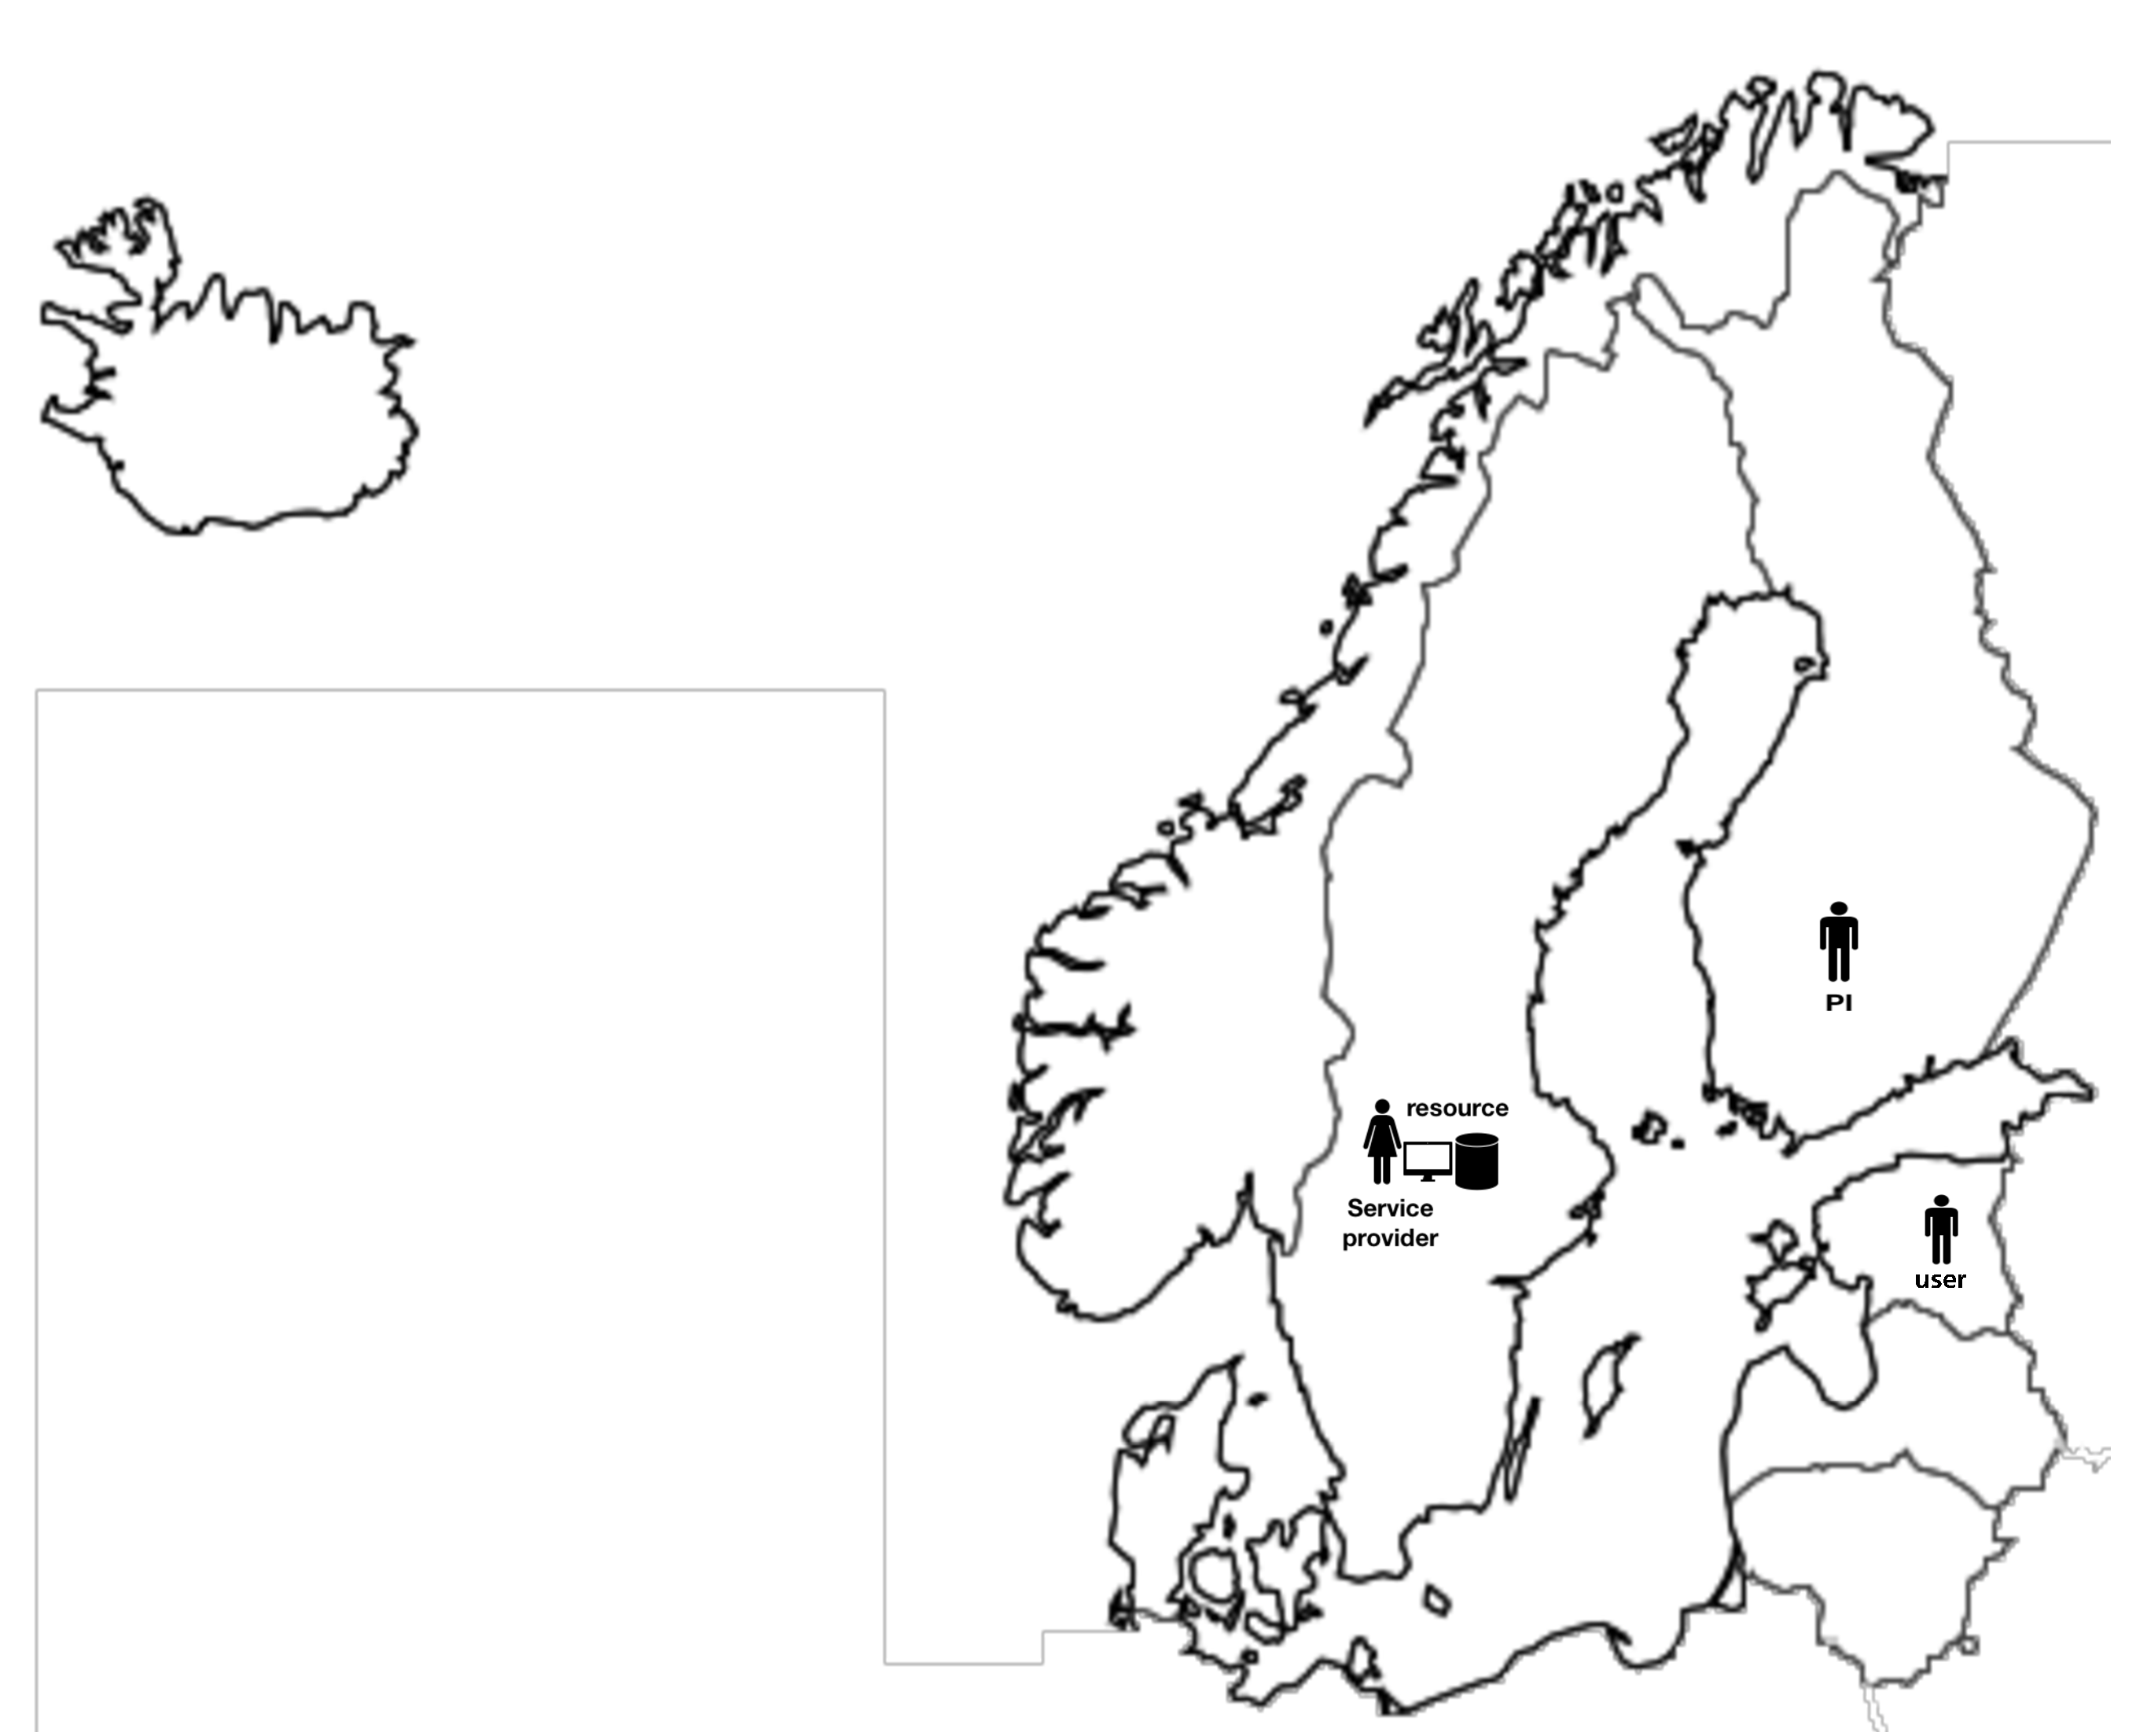
\includegraphics[width=10cm]{PI_EU_User_EU.pdf}
\caption{PI is active in an EU country and user is active within the EU.}\label{fig:eu_eu}
\end{figure}

\begin{figure}[!ht]
\centering
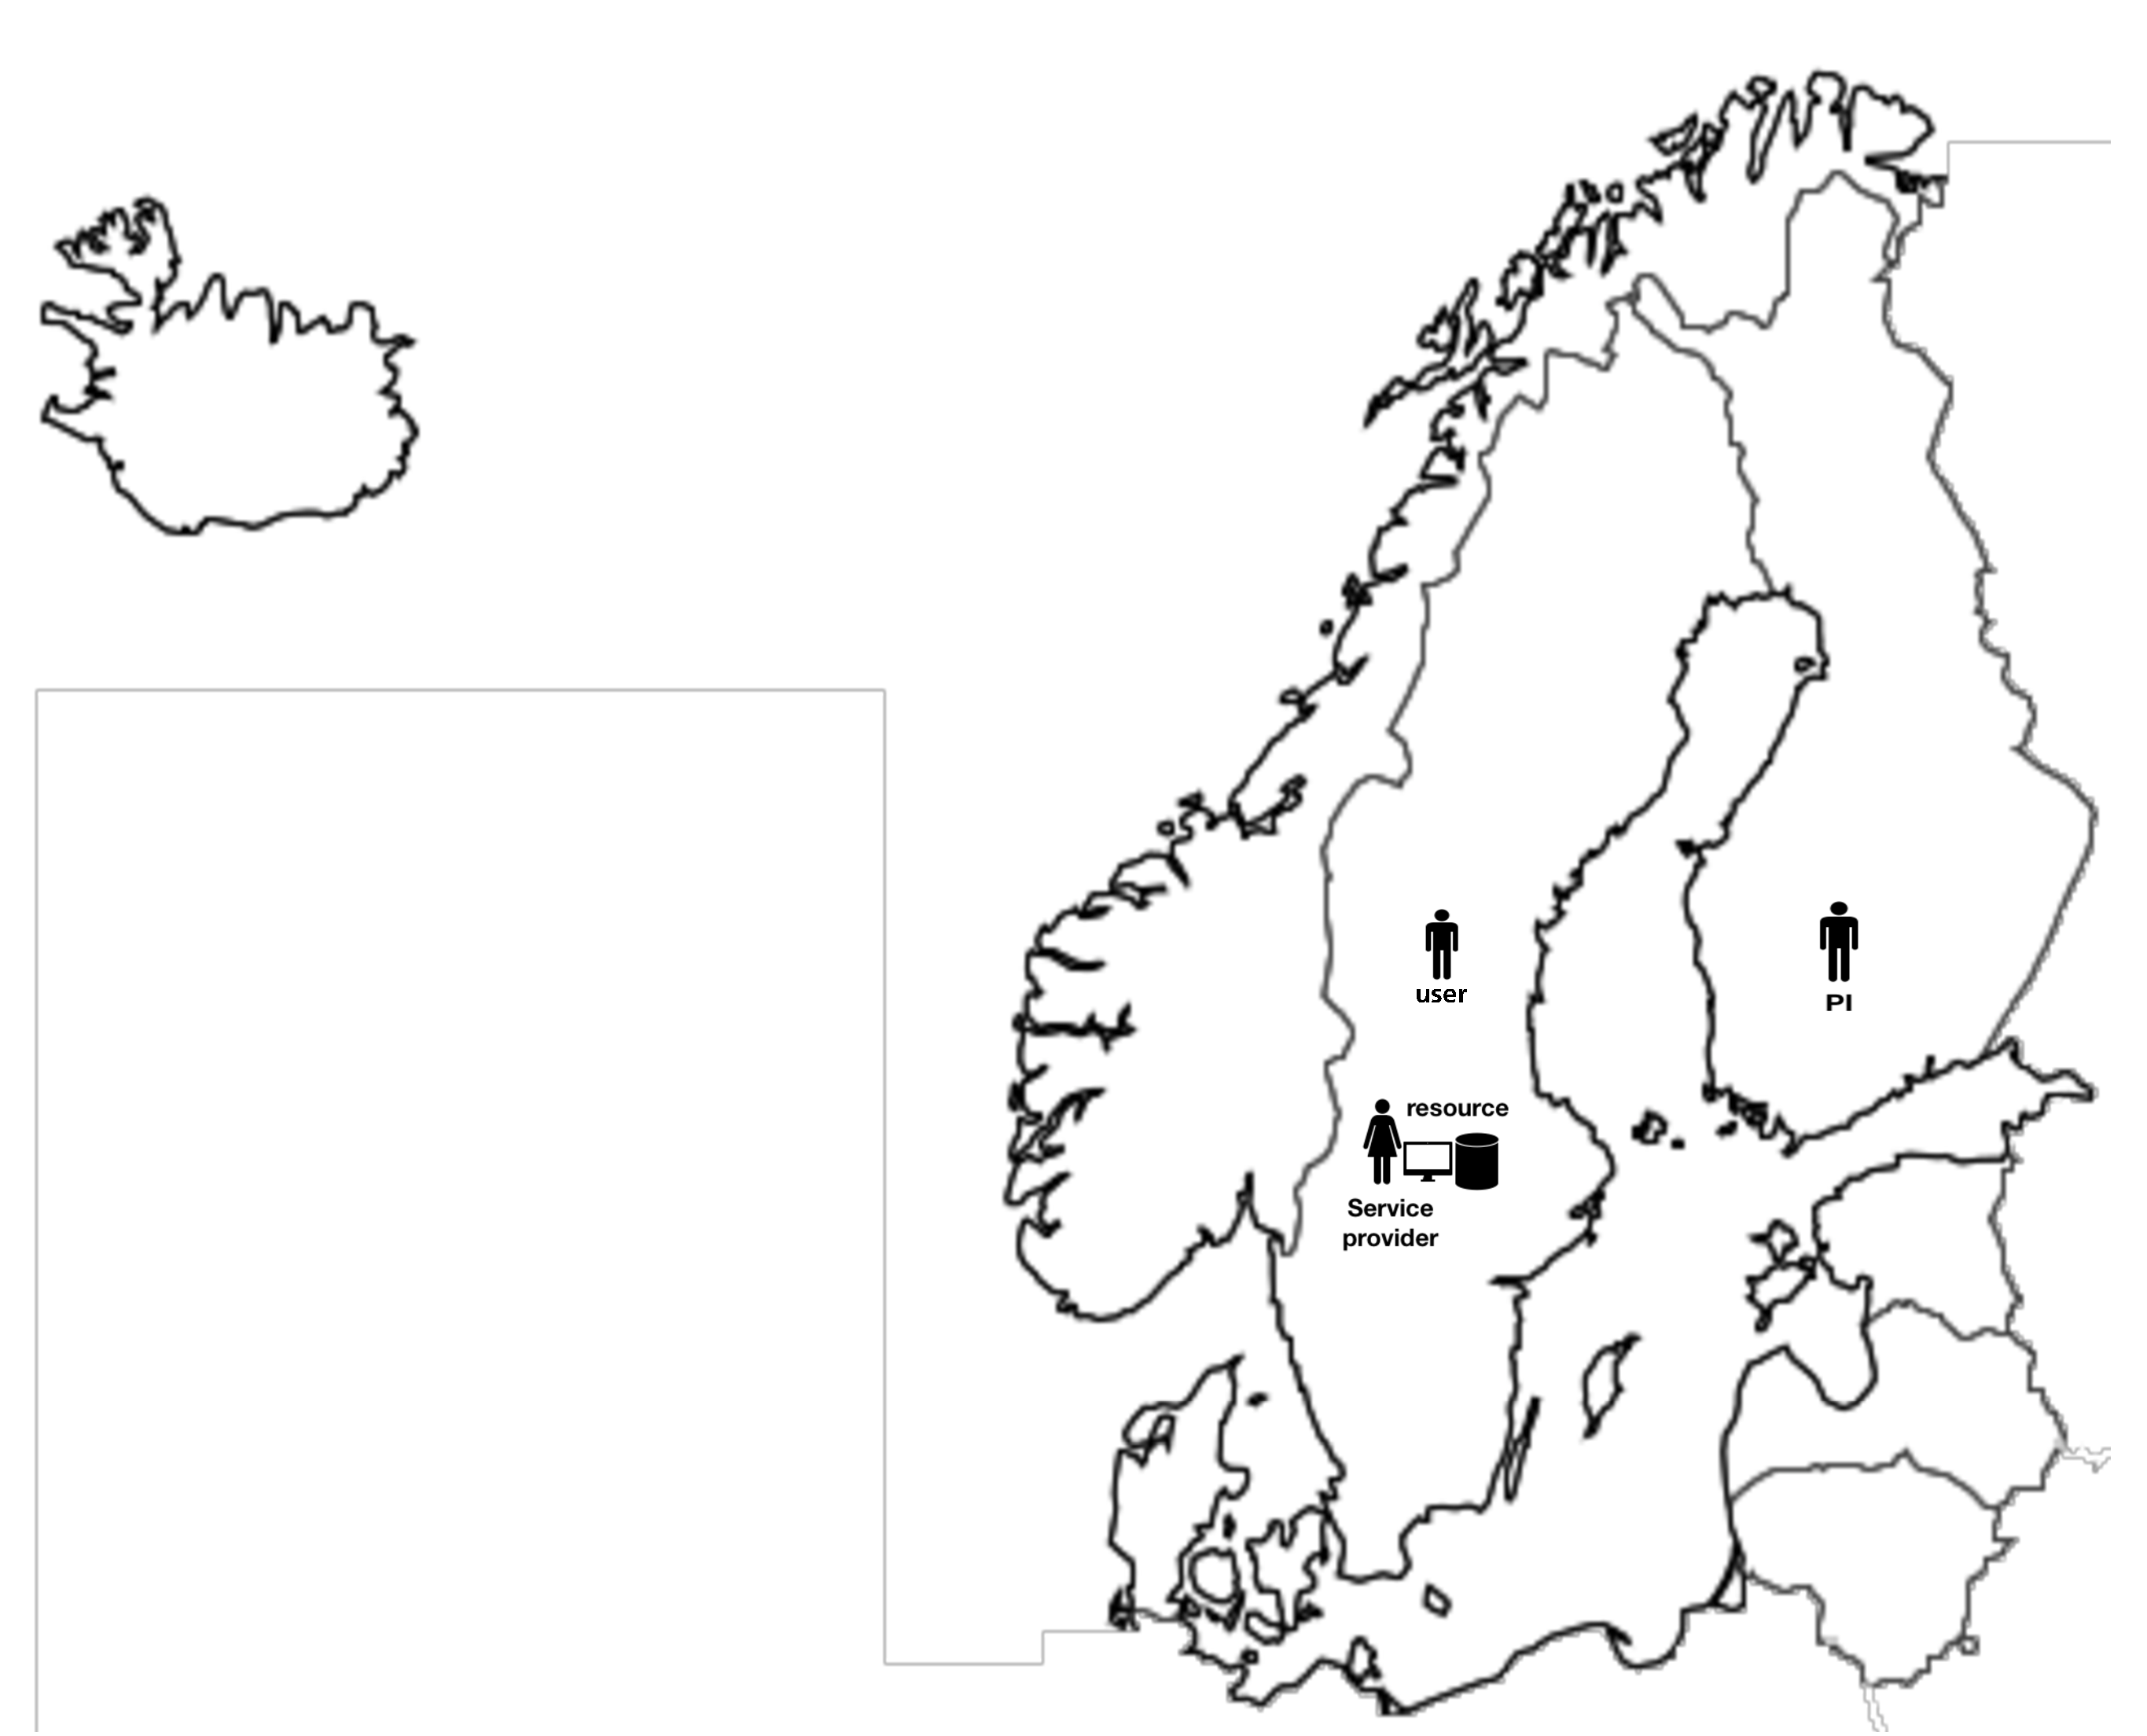
\includegraphics[width=10cm]{PI_EU_User_National.pdf}
\caption{PI is active in an EU country and user is active in the same country as the computational resource.}\label{fig:eu_nat}
\end{figure}

\begin{figure}[!ht]
\centering
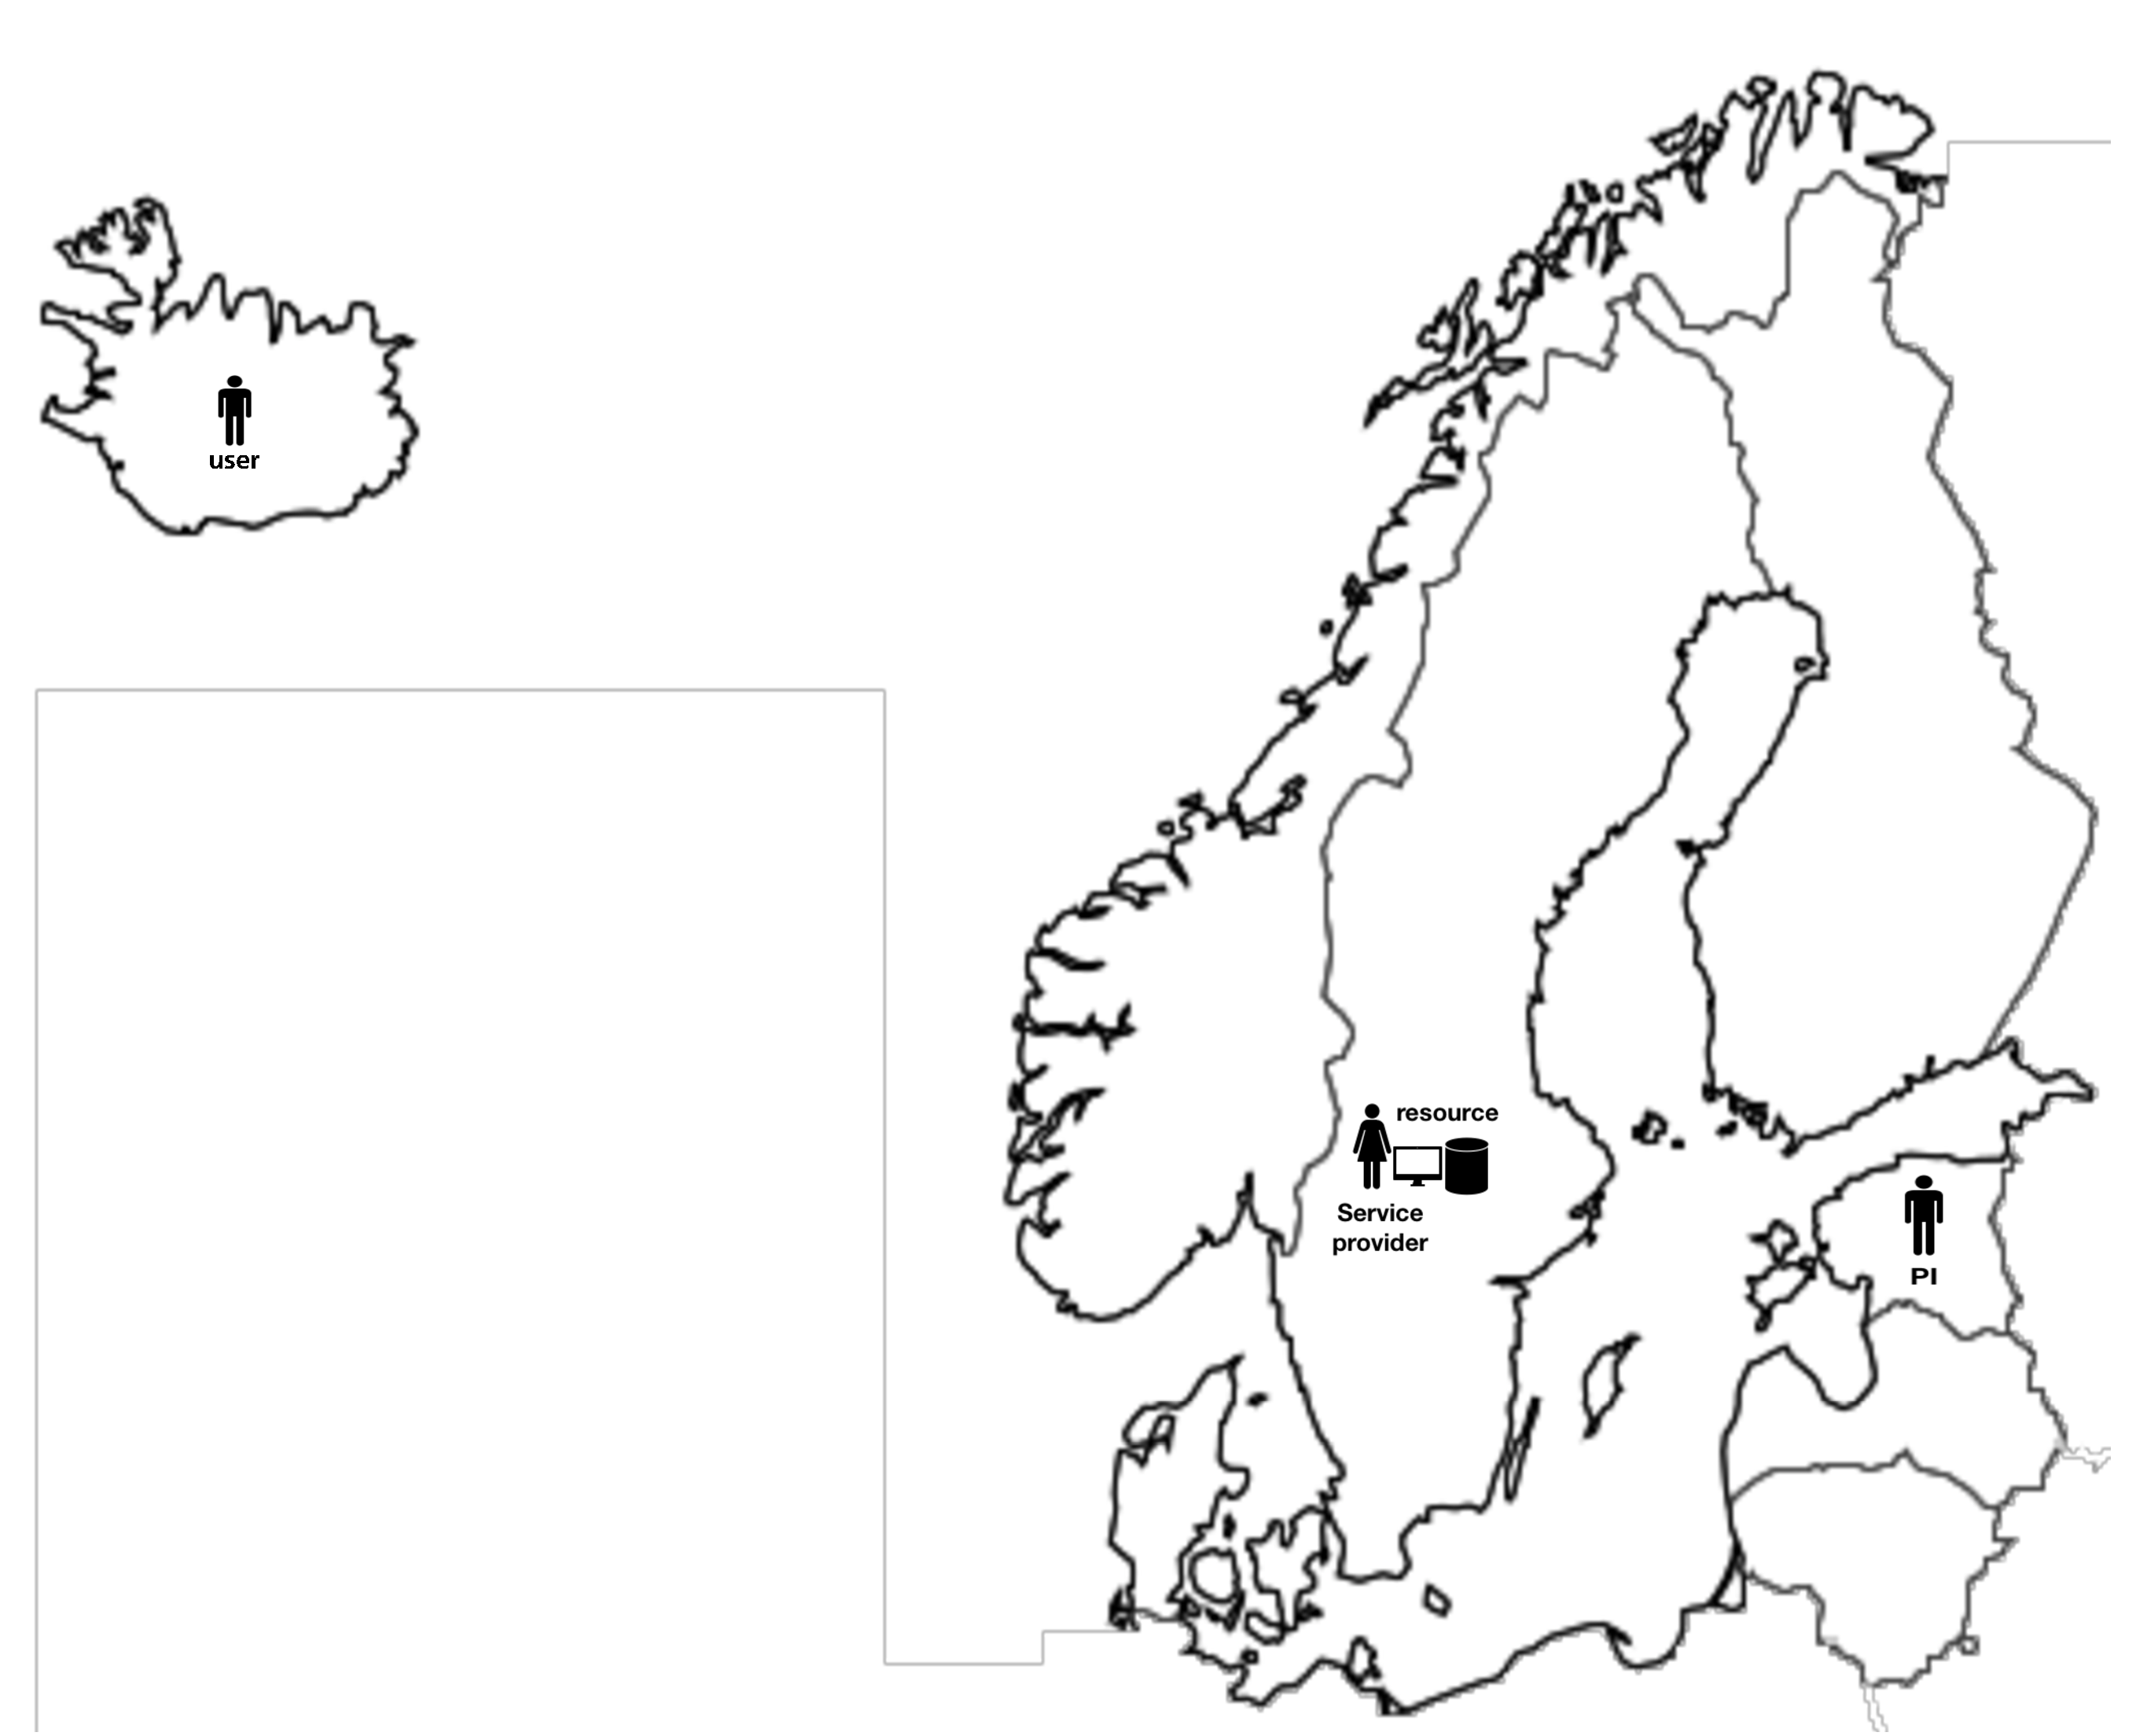
\includegraphics[width=10cm]{PI_EU_User_EEA.pdf}
\caption{PI is active in an EU country and user is active within an EFTA country.}\label{fig:eu_eaa}
\end{figure}

\begin{figure}[!ht]
\centering
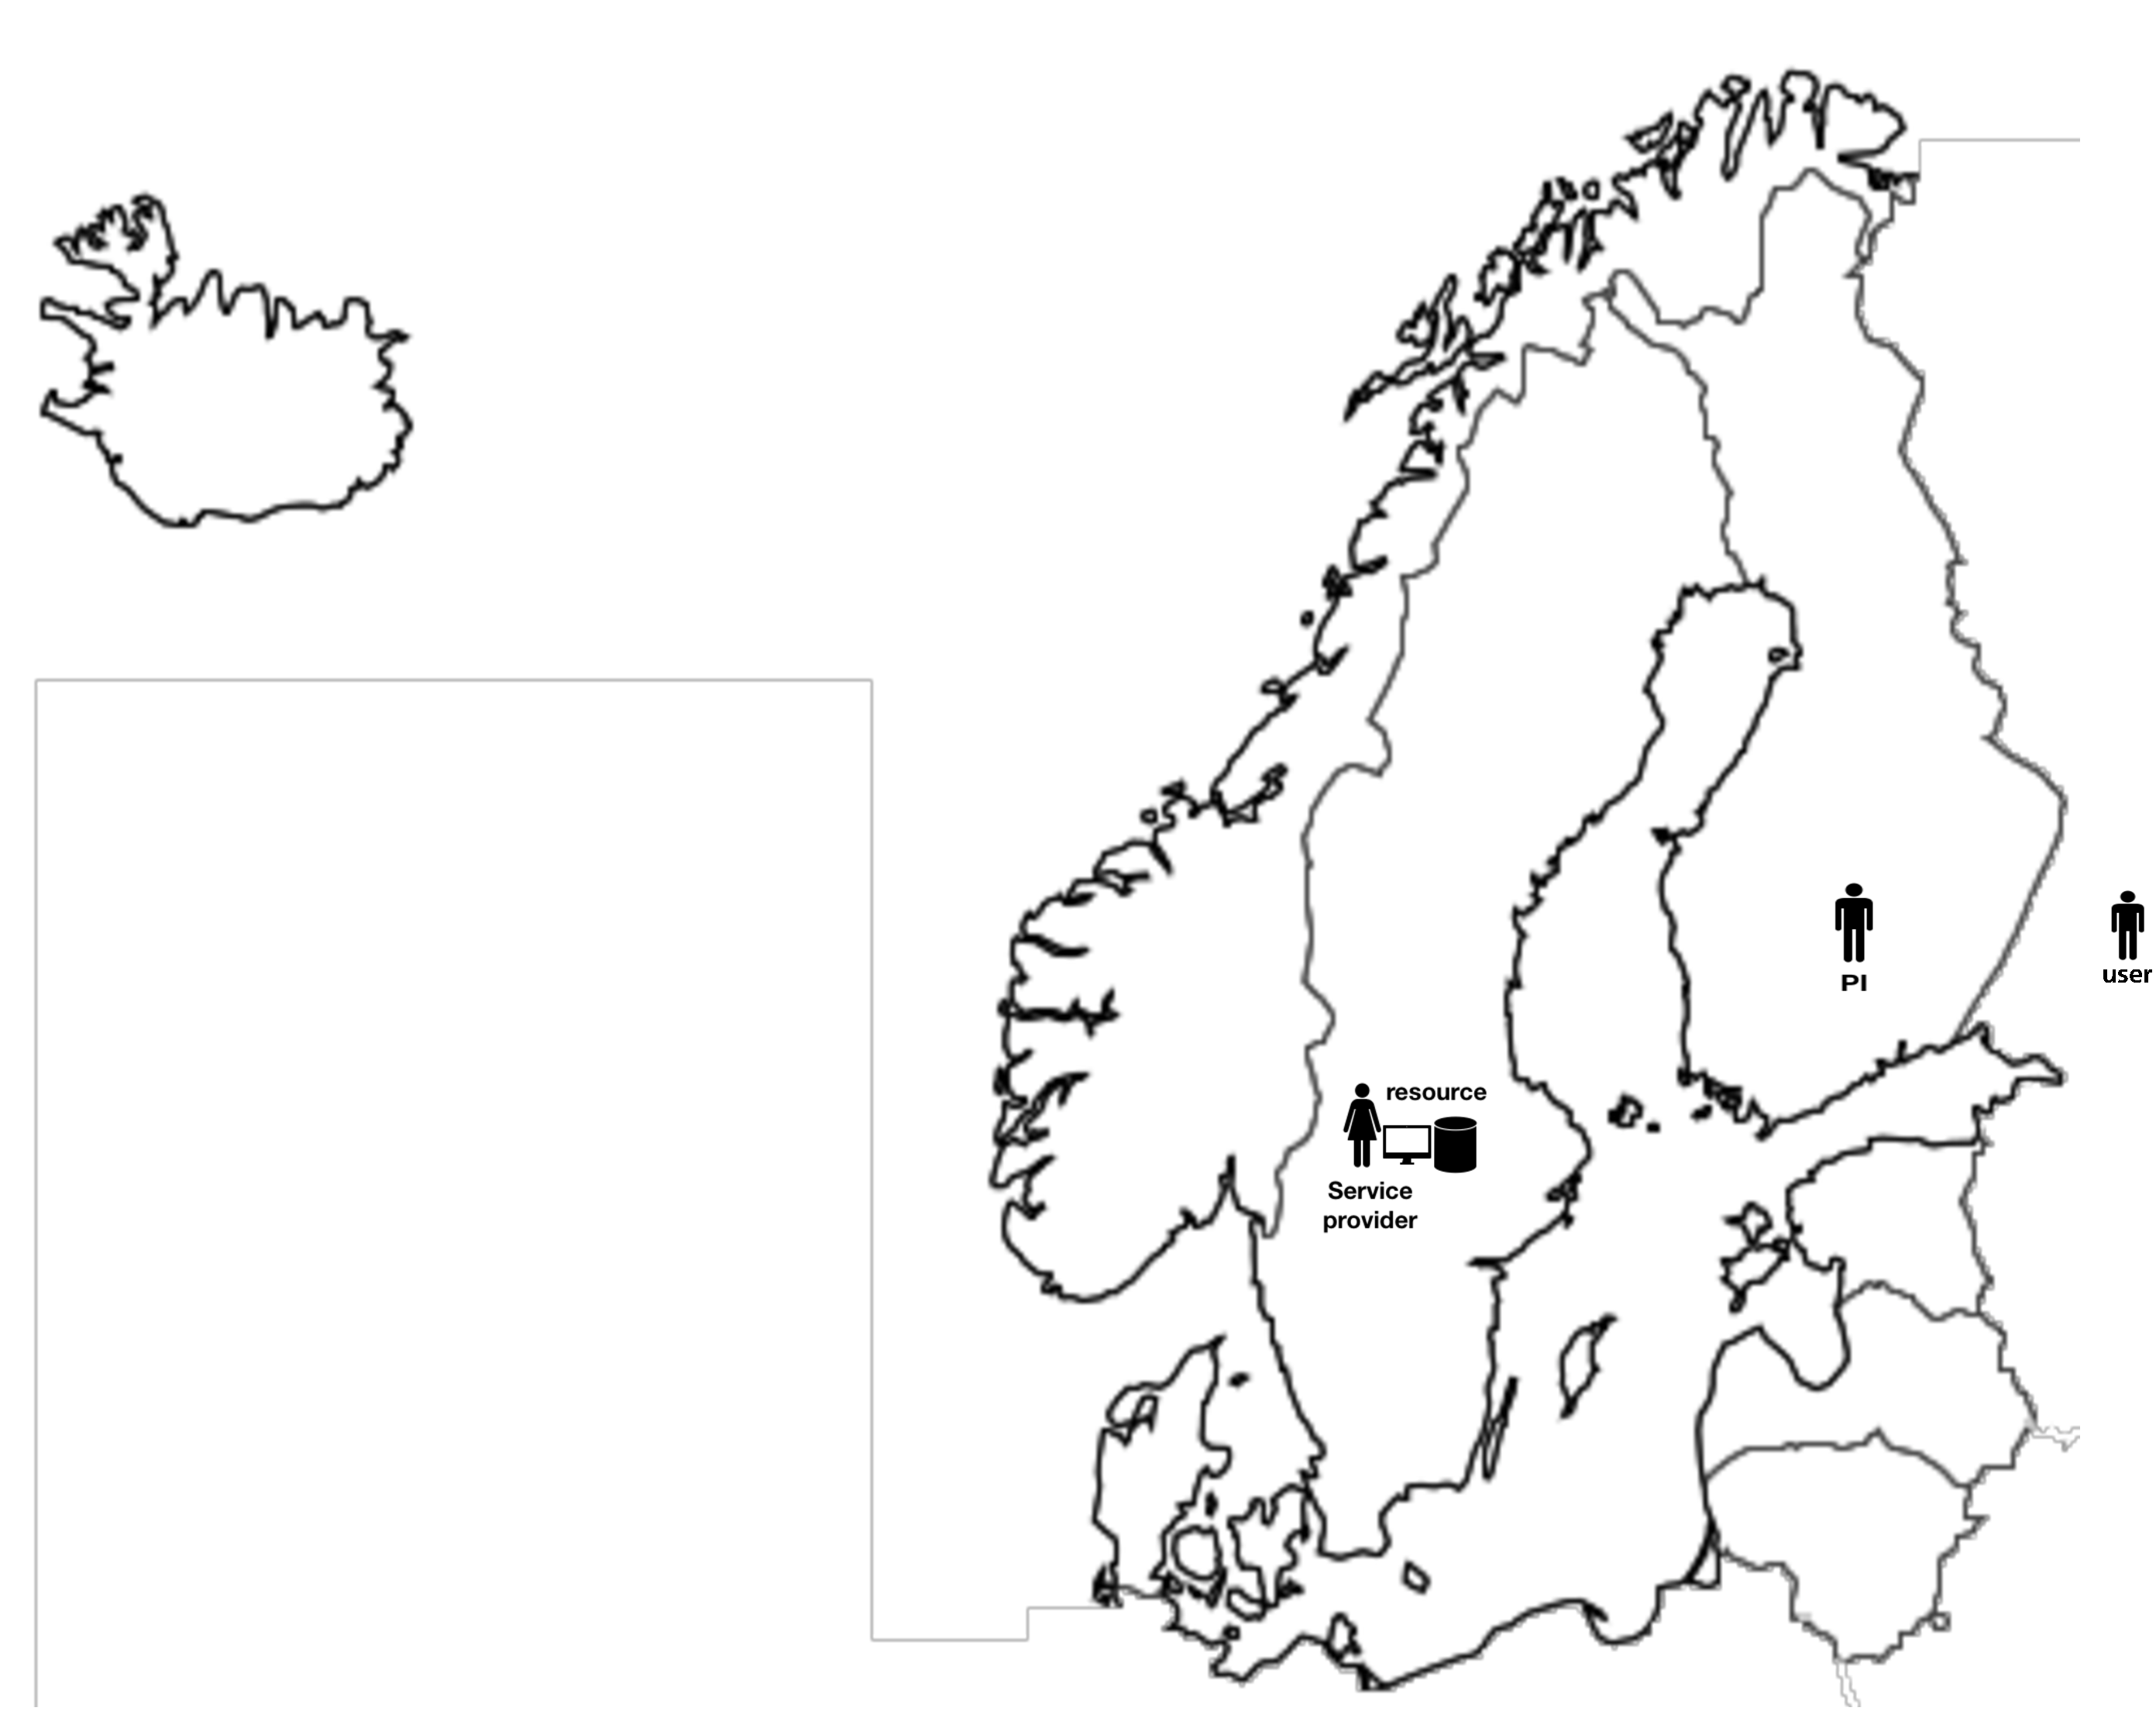
\includegraphics[width=10cm]{PI_EU_User_Non_EU.pdf}
\caption{PI is active in an EU country and user is active outside the EEA.}\label{fig:eu_non}
\end{figure}

\begin{figure}[!ht]
\centering
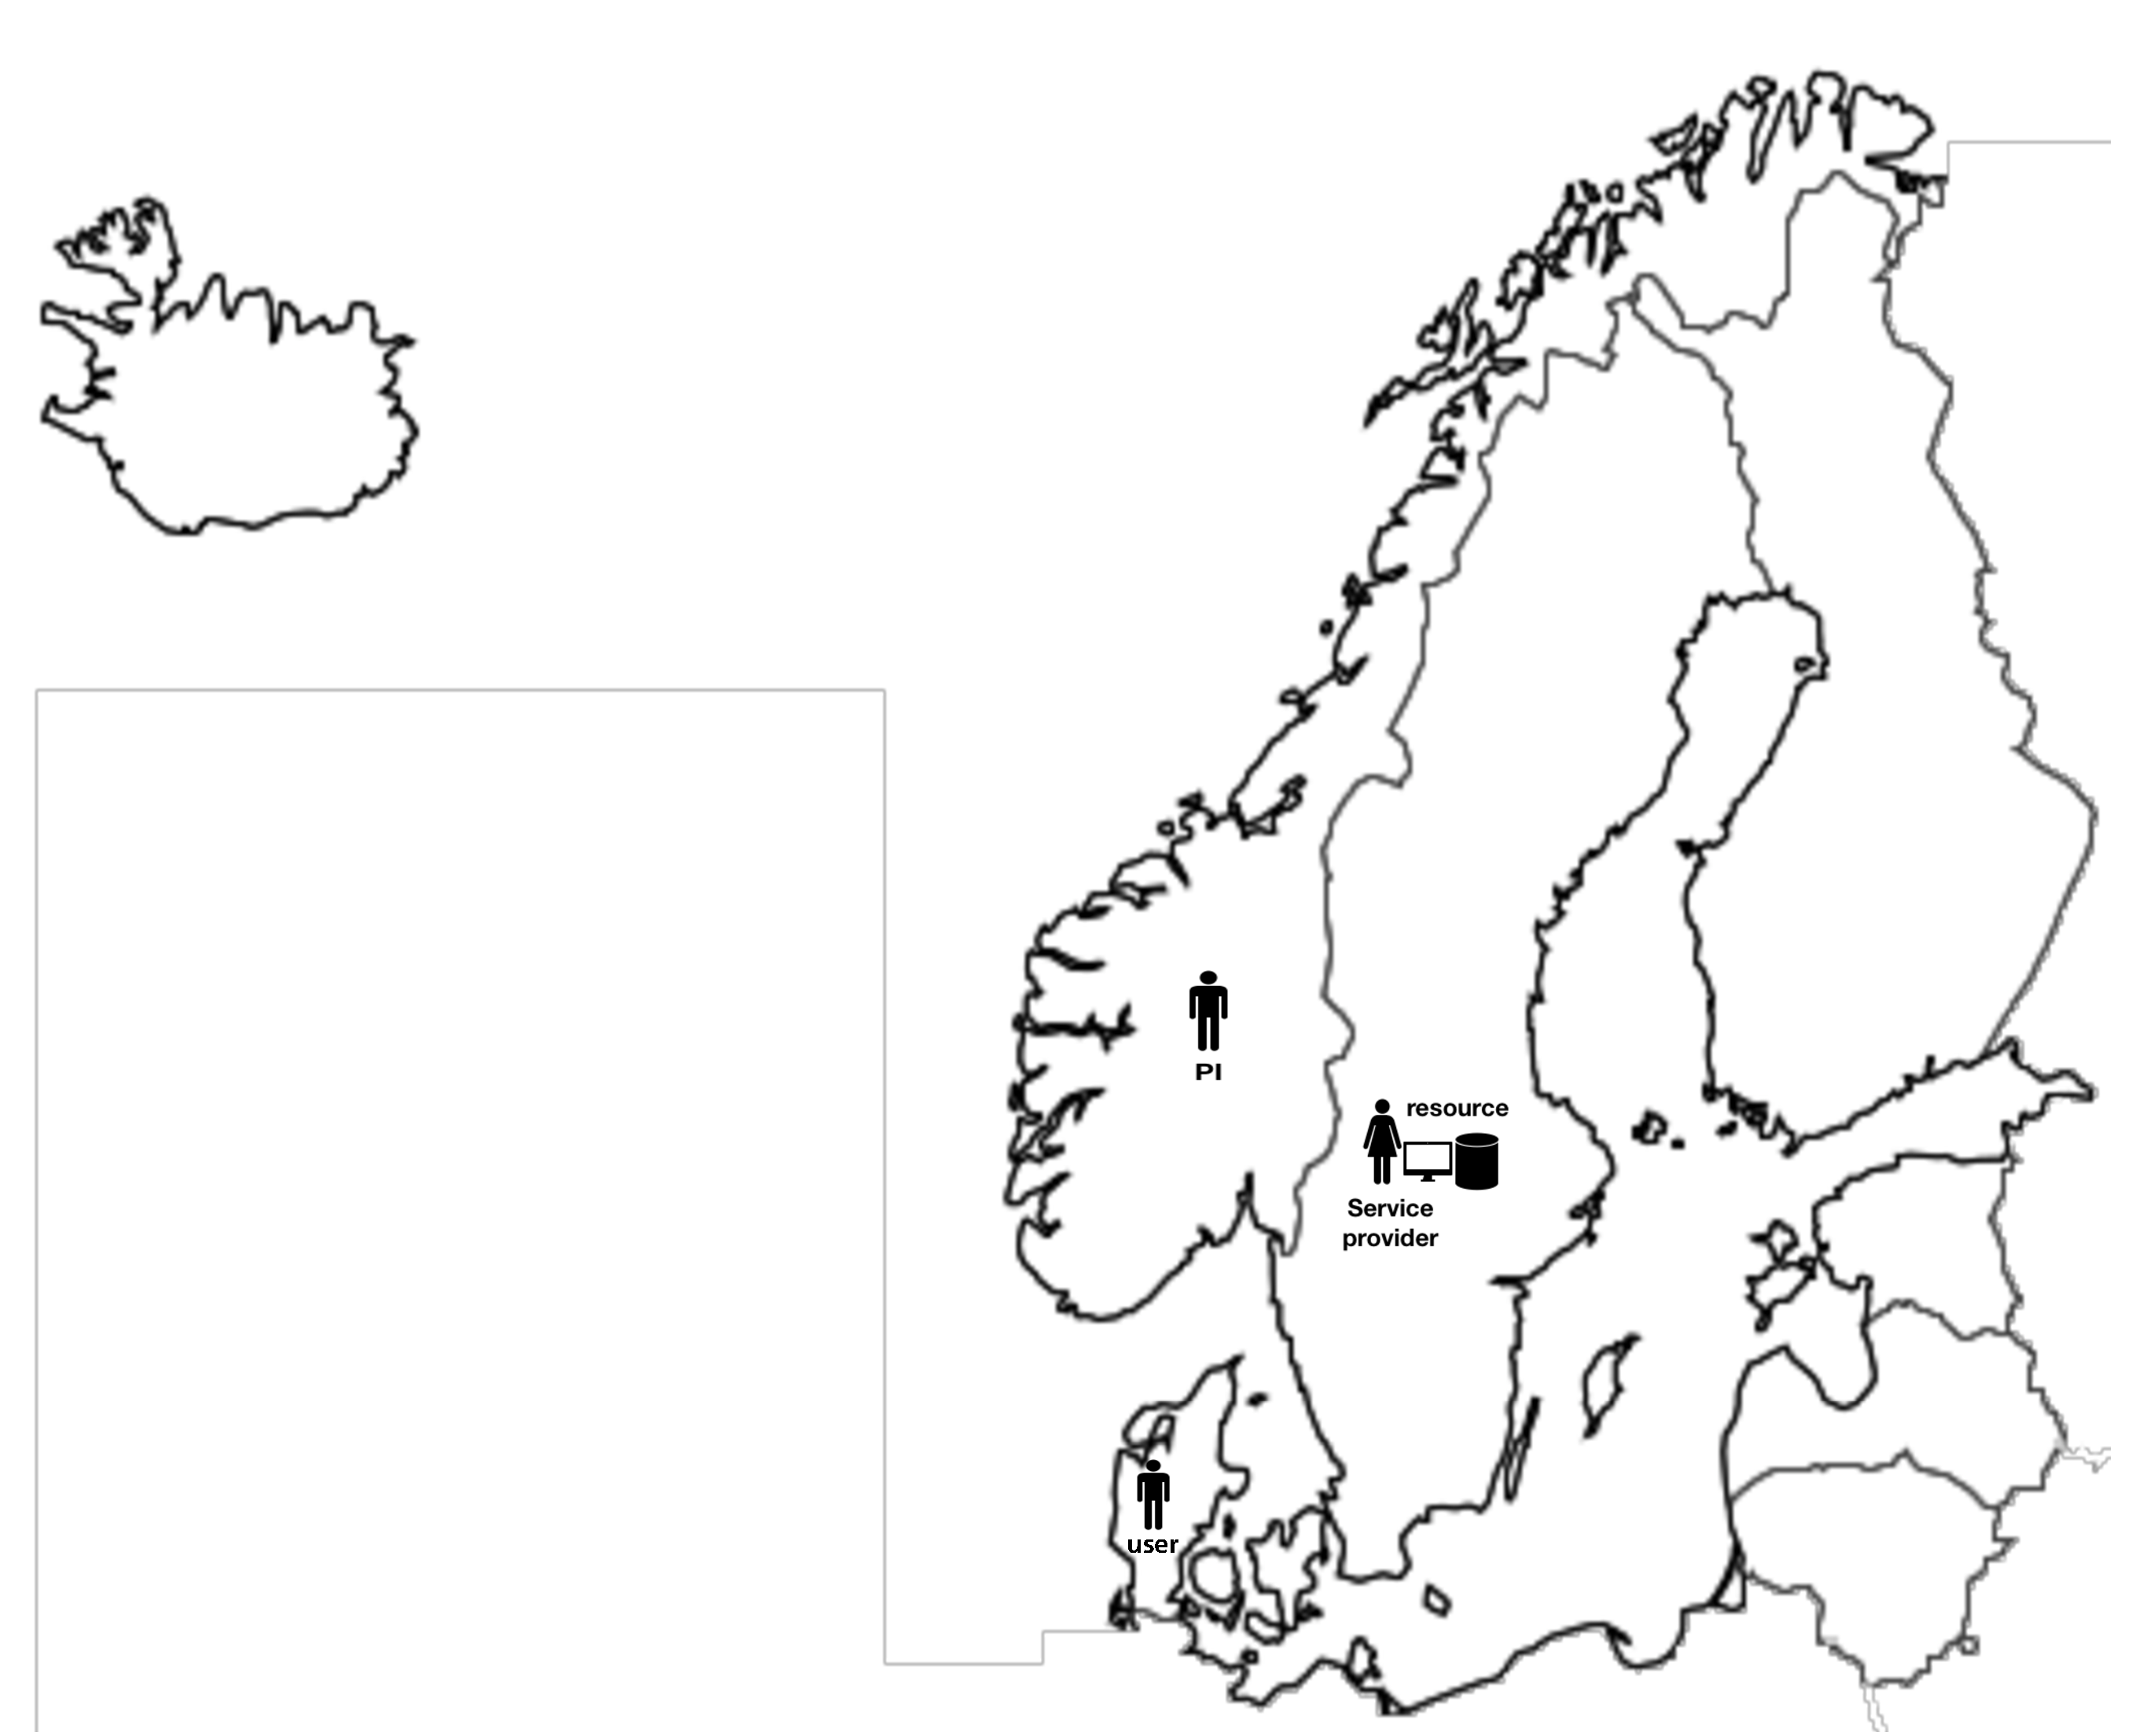
\includegraphics[width=10cm]{PI_EAA_User_EU.pdf}
\caption{PI is active in an EFTA country and user is active within the EU.}\label{fig:eaa_eu}
\end{figure}

\begin{figure}[!ht]
\centering
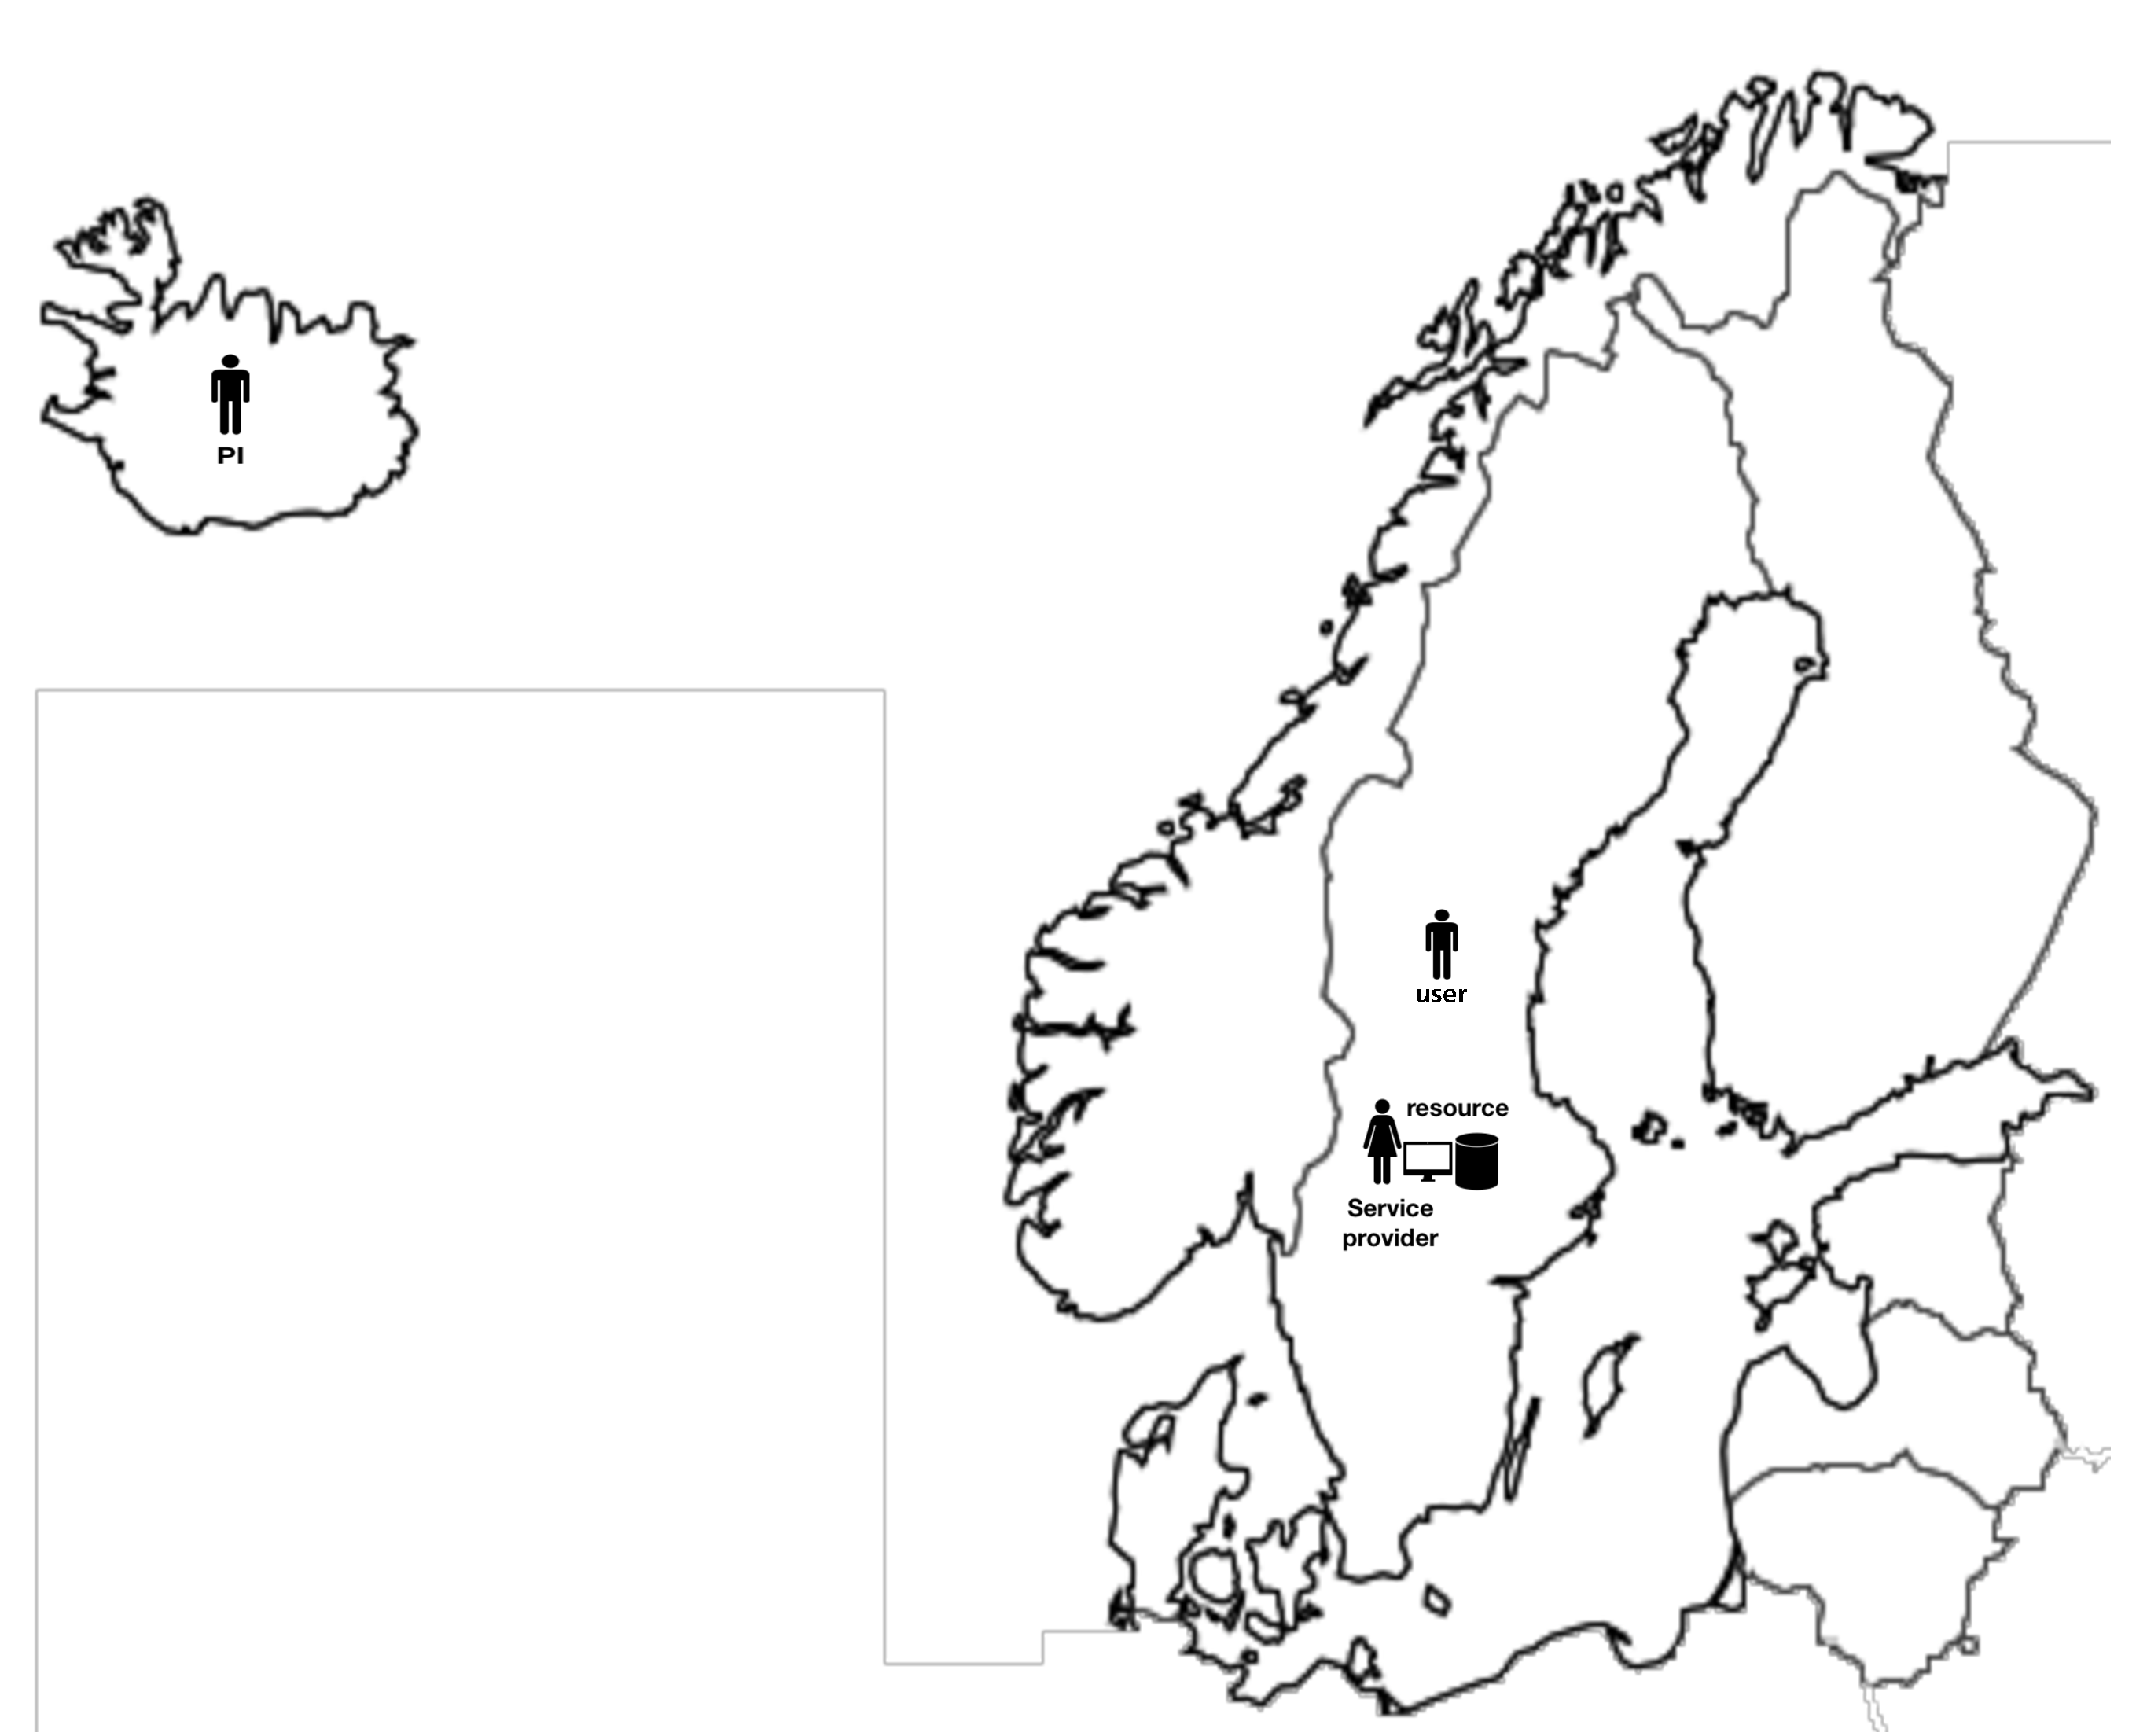
\includegraphics[width=10cm]{PI_EAA_User_National.pdf}
\caption{PI is active in an EFTA country and user is active in the same country as the computational resource.}\label{fig:eaa_nat}
\end{figure}

\begin{figure}[!ht]
\centering
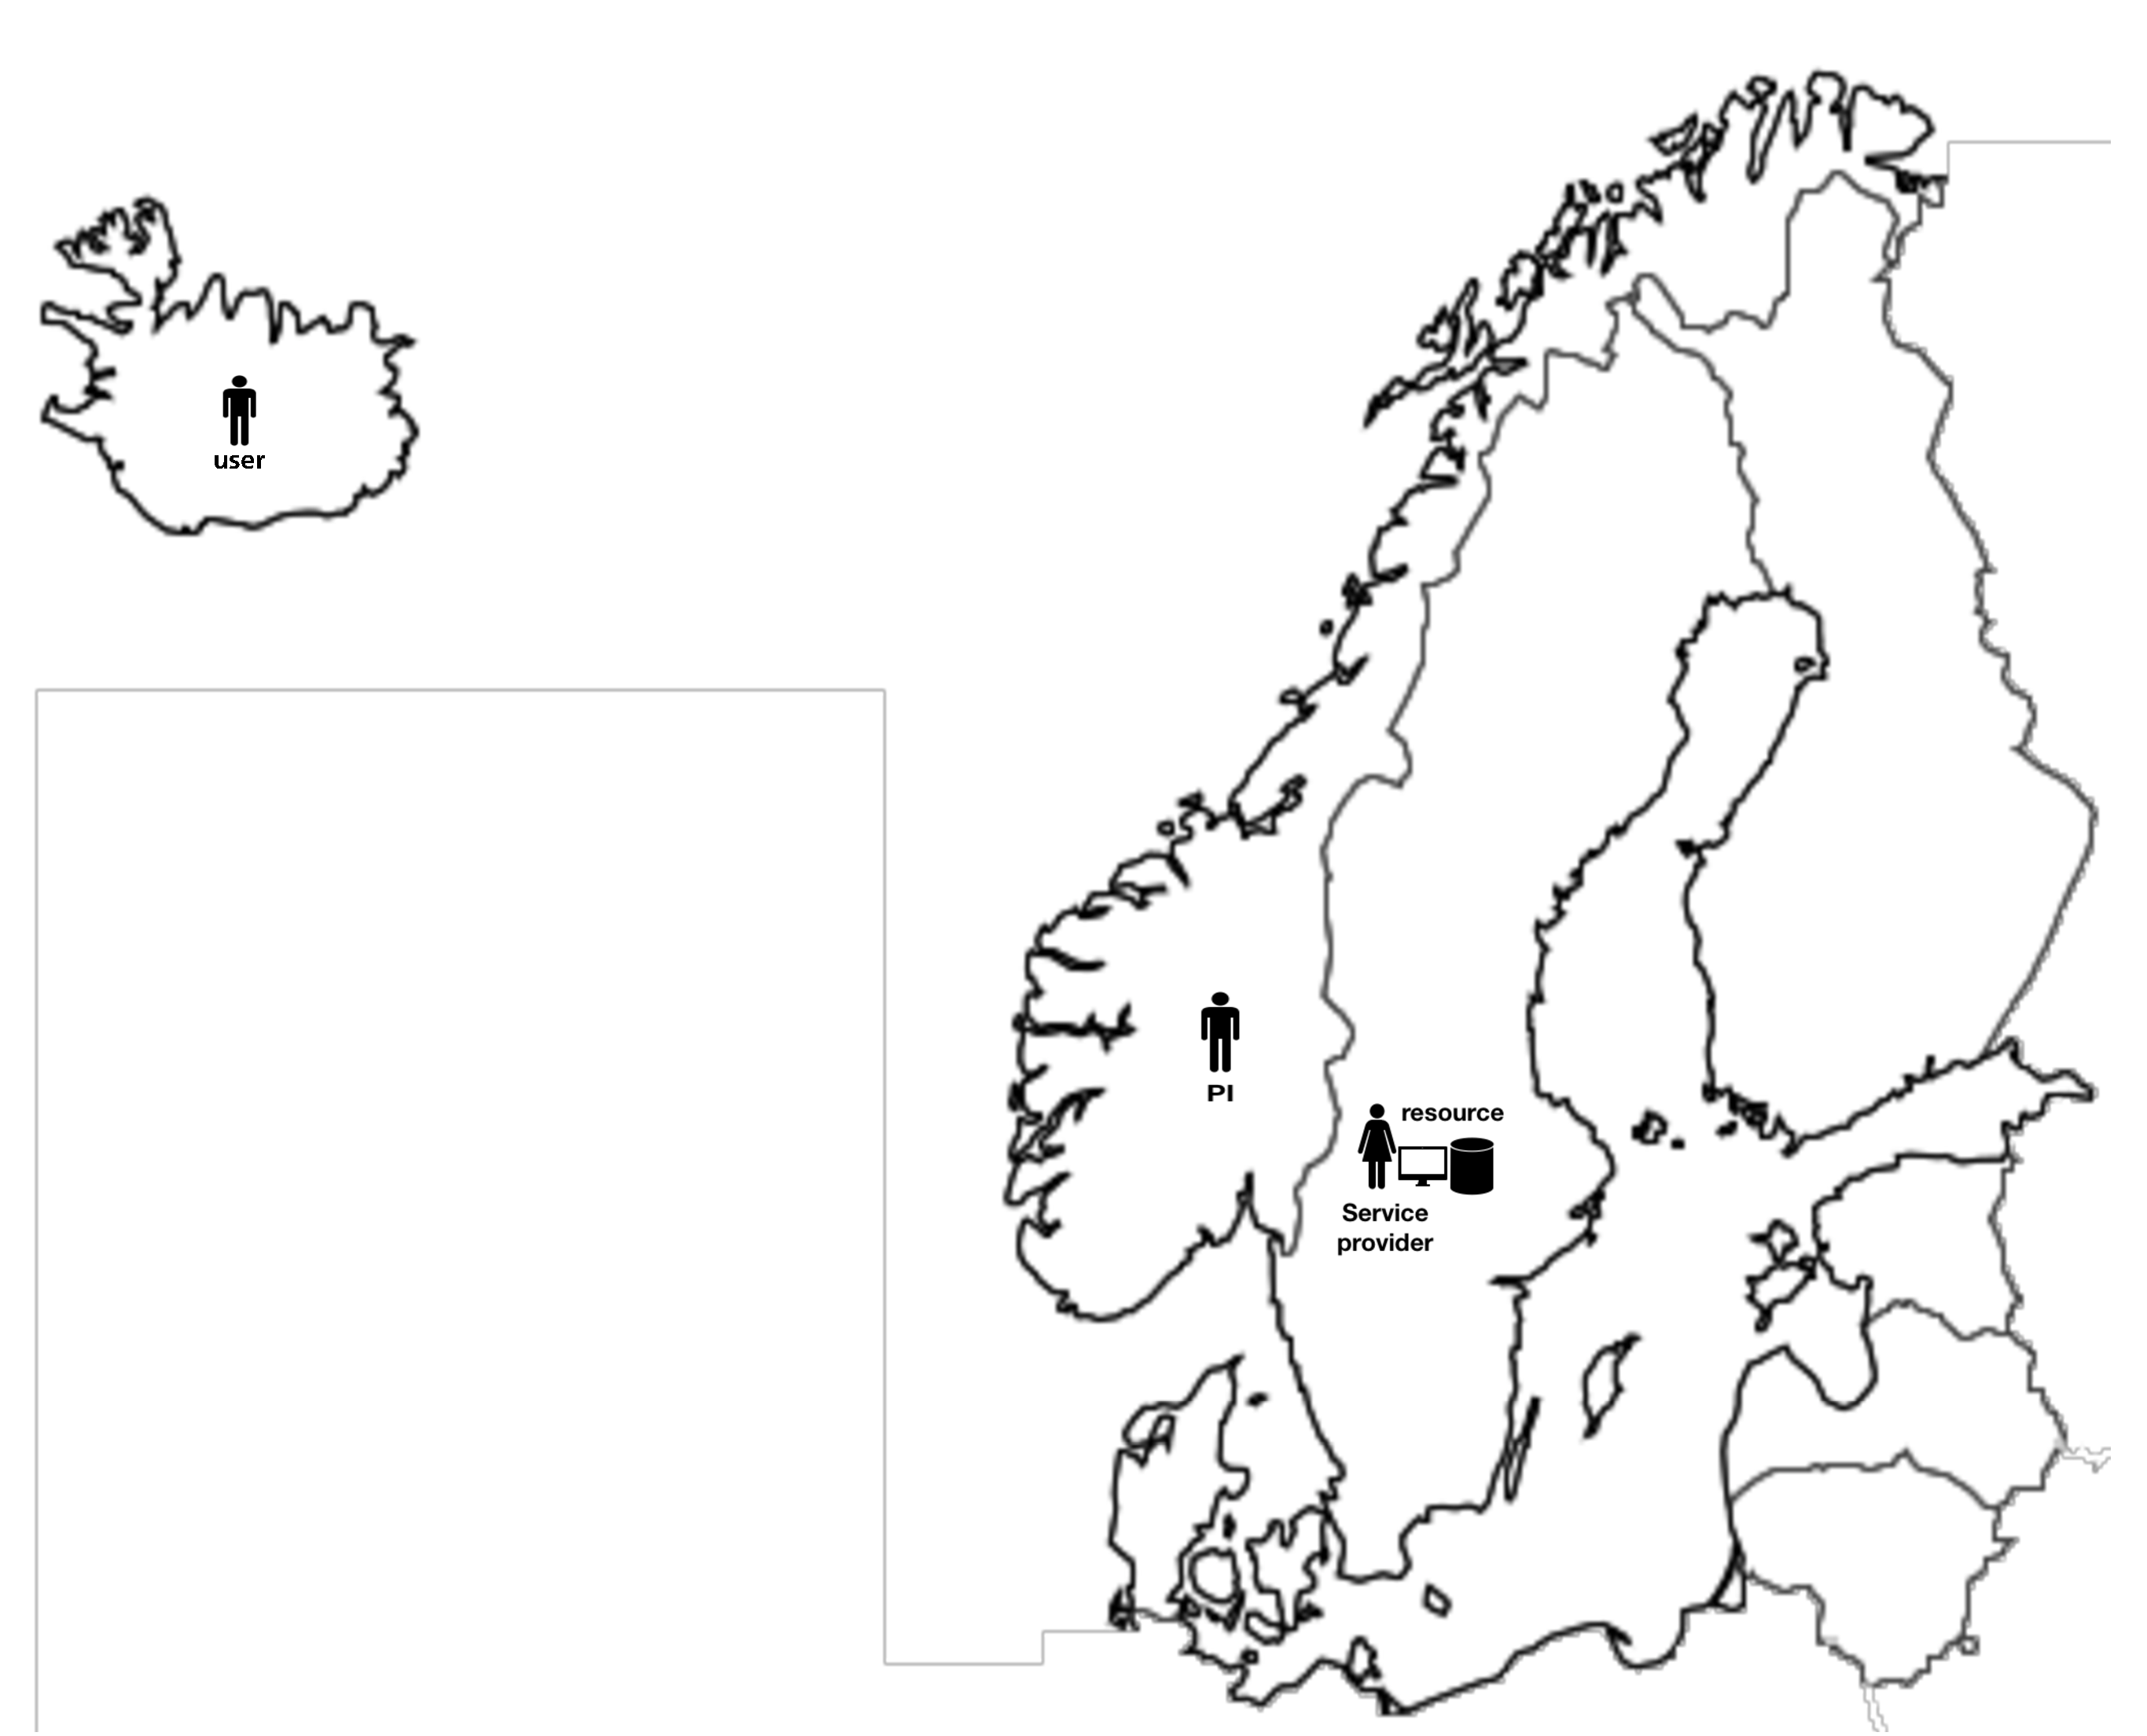
\includegraphics[width=10cm]{PI_EAA_User_EEA.pdf}
\caption{PI is active in an EFTA country and user is active within an EFTA country.}\label{fig:eaa_eaa}
\end{figure}

\begin{figure}[!ht]
\centering
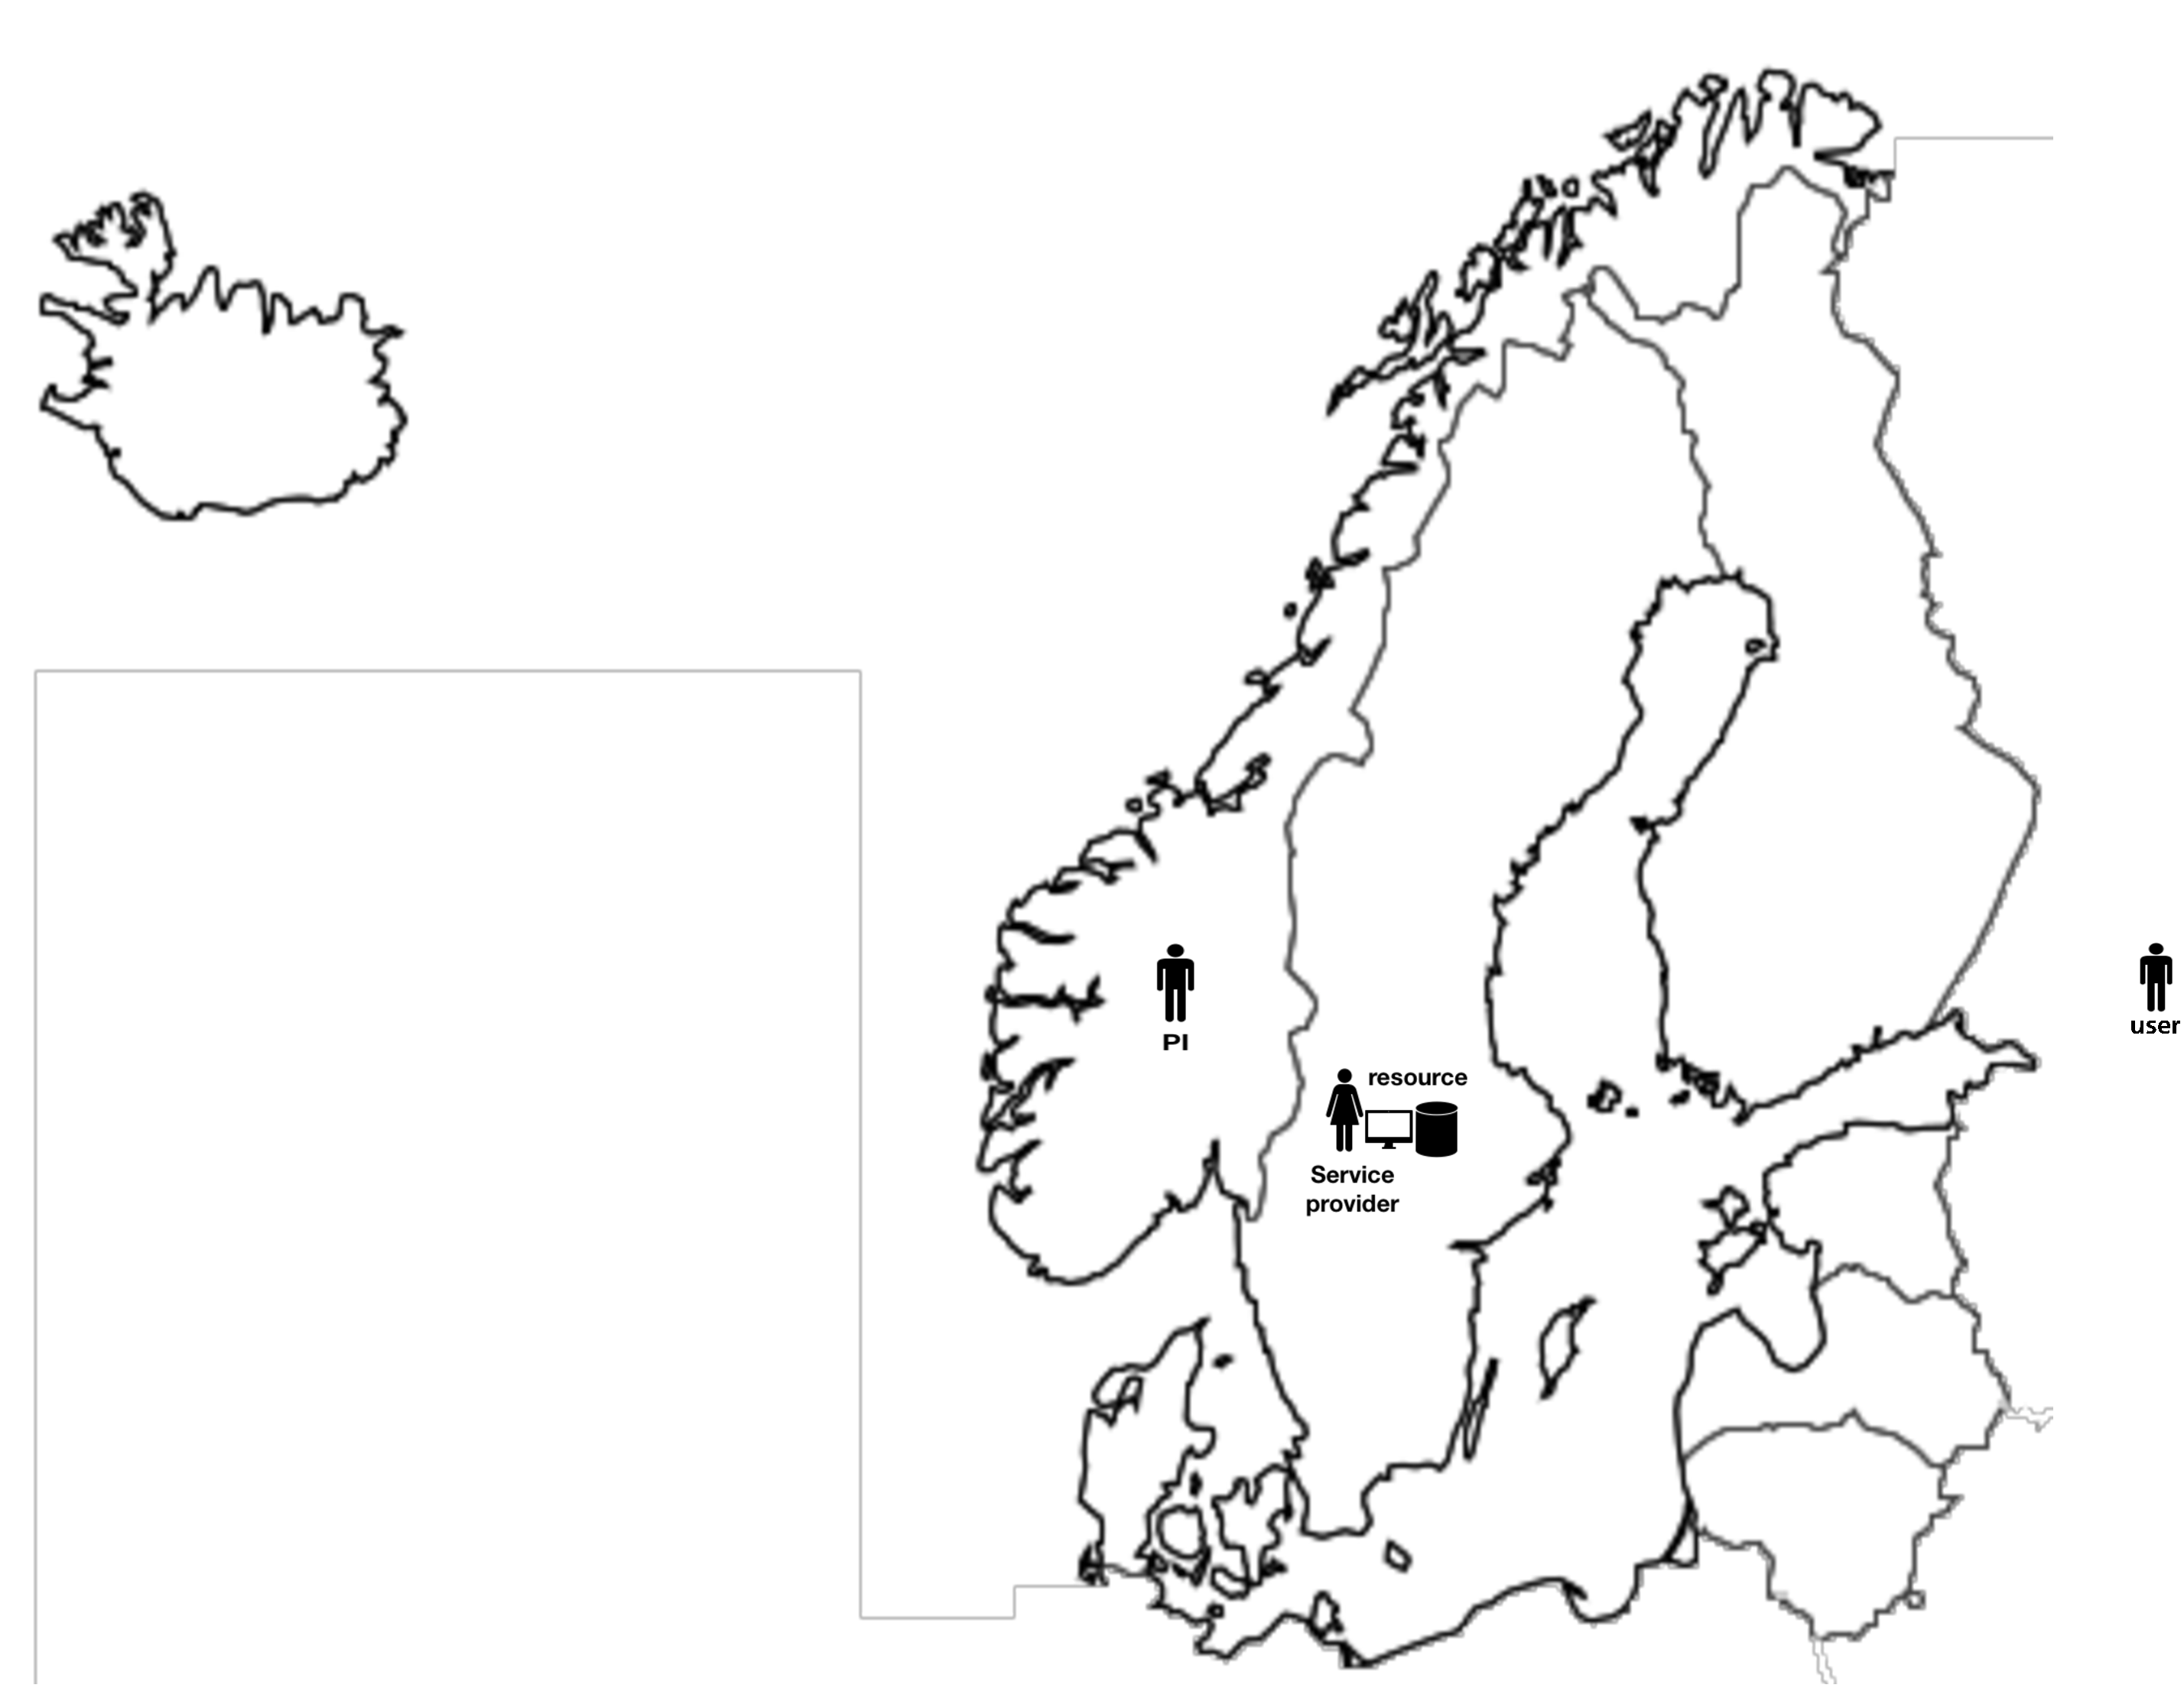
\includegraphics[width=10cm]{PI_EAA_User_Non_EU.pdf}
\caption{PI is active in an EFTA country and user is active outside the EEA.}\label{fig:eaa_non}
\end{figure}

\section{Policies}
\begin{itemize}
    \item []
These preconditions must be evaluated in close interaction with management of national provider organisations and resource allocation committees. Should these preconditions be met, a framework agreement can be put in place with the national providers.
\end{itemize}
\subsection{Preconditions by participating country}
\label{sec-precond}

The preconditions for organizations and users to access shared resources
offered by the participating providers are given below.
The definition of ``Citizen of country subject to sanctions by the EU" is given by~\cite{eu-sanctions}.
The sanctions that affect the \dell project are illustrated in~\cite{eu-sanctions-guide} and include: Restrictions on services; Dual-use goods; Restrictions on goods.
The definition of these restrictions vary from country to country but, in general, a \einfra resource cannot be accessed by a citizen of an embargoed country if the resources could be used in the pursuit of banned activities.

\subsubsection{Denmark}
\begin{itemize}
    \item []
Denmark provides access to two separate resources (\textbf{Abacus 2.0}~\cite{abacus} and \textbf{Computerome}~\cite{computerome}) where Computerome can only be used for Life Science projects. 

    \item[] Use cases: 
    \begin{itemize}
        \item[] 
    For the scenarios identified in Section~\ref{sec:usecase} the eligibility of a customer e.g. an organisation or company, to use the resources are as shown in table \ref{tab:DK_use_cases}.
    \end{itemize}
    \begin{table}[!h]
        \centering
        \begin{tabular}{|l|c|}
        \hline
             & Valid customer  \\
        \hline
Research/public organisation in the same country & OK \\
        \hline
Research/public organisation in the EU & OK \\
        \hline
Research/public organisation in an EFTA country & OK \\
        \hline
Research/public organisation outside the EEA & OK\\
        \hline
Private company in own country & OK \\
        \hline
Private company in Europe    & OK \\
        \hline
Private company outside the EEA & OK \\
        \hline 
        \end{tabular}
        \caption{User access cases (Denmark).}
        \label{tab:DK_use_cases}
    \end{table}
    
    \item[]Eligibility:
    \begin{itemize} 
        \item[]\textbf{Abacus 2.0}: Open to all researchers in Denmark, and all academic users. Applicants for any kind of allocation schemes must hold at least the position of postdoc within their institution. PhD students request access in consultation with, and under the auspices of, their supervisor. Access to the facility is not free. 
        
        \item[]\textbf{Computerome}: Available to (mostly Danish) academia and industry users.
        Access to the facility is not free.
        \item[]The eligibility of a users access to the resources is outlined in table \ref{tab:DK_user_elegibility}
        \begin{table}[!h]
       \centering
        \begin{tabular}{|l|c|c|}
            \hline
        & Abacus 2.0 (SDU) & Computerome (DeIC) \\
        \hline
      Same country national  &   OK  &  OK \\
        \hline
        EU citizen      &   OK  &  OK  \\
            \hline
            Citizen from outside EU	        &   OK  &  OK  \\
            \hline
            Citizen of country subject to sanctions by the EU & No & No \\
            \hline
            \end{tabular}
        \caption{Eligibility of users (Denmark).}
        \label{tab:DK_user_elegibility}
    \end{table}

    \end{itemize} 
    \item[]Access:
    \begin{itemize} 
        \item[]\textbf{Abacus 2.0}: All researchers – except researchers affiliated with Aarhus University (AU) and Aalborg University (AAU) need to request their HPC account online on website. Researchers affiliated to AU and AAU request their local HPC coordinator for access to the facility.
        \item[]\textbf{Computerome}: Access requests should be sent via E-Mail to Computerome support and must include organisation E-mail and mobile phone number for the requested account(s).
        \item[]User access validation for the respective resources is performed as stated in Table~\ref{tab:DK_user_acc_val}.
        %
 Note that~\href{https://wayf.dk}{WAYF}~\cite{wayf} (Where Are You From)
 is Denmark's identity federation for research and higher education.
\end{itemize} 
    \begin{table}[!h]
       \centering
        \begin{tabular}{|l|c|c|}
            \hline
        & Abacus 2.0 (SDU) & Computerome (DeIC) \\
        \hline
      Same country national  & WAYF  
      & Institutional email \\
        \hline
        EU citizen      &  Institutional email + EduGAIN   & Institutional email \\
            \hline
            Citizen from outside EU	        &  Institutional email + EduGAIN   & Institutional email \\
            \hline
            \end{tabular}
        \caption{Means of user identity validation (Denmark).}
        \label{tab:DK_user_acc_val}
    \end{table}
\end{itemize} 

\subsubsection{Estonia}
\begin{itemize}
    \item []
The Estonian Scientific Computing Infrastructure (ETAIS)~\cite{etais} provides access to one resource (\textbf{Rocket})~\cite{etais-rocket}. 
For the scenarios identified in Section~\ref{sec:usecase} the eligibility of a customer e.g. an organisation or company, to use the resources are as shown in table~\ref{tab:ET_use_cases}.
\end{itemize}
\begin{itemize}
\item[] Use cases:
    \begin{table}[!h]
        \centering
        \begin{tabular}{|l|c|}
        \hline
             & Valid customer  \\ 
        \hline
 Research/public organisation in the same country & OK \\
       \hline 
Research/public organisation in the EU &  OK\\
        \hline
Research/public organisation in an EFTA country & OK\\
        \hline
Research/public organisation outside the EEA & depends\\
        \hline
Private company in own country & OK\\
        \hline
Private company in Europe    & OK\\
        \hline
Private company outside the EEA & depends\\
        \hline 
        \end{tabular}
        \caption{User access cases (Estonia).}
        \label{tab:ET_use_cases}
    \end{table}
    
\item[]Eligibility:
\begin{itemize} 
\item[] The main aim of ETAIS is to serve Estonian students and researchers. 
ETAIS also provide services for private organisations. 
The eligibility of a users access to the resources is outlined in Table~\ref{tab:ET_user_elegibility}.
\begin{table}[!h]
    \centering
    \begin{tabular}{|l|c|}
        \hline
    & Rocket  \\
    \hline
  Same country national      & OK \\
    \hline
    EU citizen       &  OK\\
        \hline
        Citizen from outside EU	         &  OK\\
        \hline
        Citizen of country subject to sanctions by the EU  & no\\
        \hline
        \end{tabular}
    \caption{Eligibility of users (Estonia).}
    \label{tab:ET_user_elegibility}
\end{table}
\end{itemize} 

\item[]Access:
\begin{itemize} 
\item[] Access to the resource is applied for via the ETAIS webpage or provided internally for ETAIS consortium members.

\begin{table}[!h]
    \centering
    \begin{tabular}{|l|c|}
        \hline
    & Rocket  \\
    \hline
  Same country national      & TARA (National eID) / eduGAIN (Estonian IdPs) \\
    \hline
    EU citizen       & TARA (eIDAS) \\
        \hline
        Citizen from outside EU	         & eduGAIN \\
        \hline
        \end{tabular}
    \caption{Means of user identity validation (Estonia).}
    \label{tab:ET_user_acc_val}
\end{table}
\end{itemize} 
\end{itemize} 

\subsubsection{Finland}
\begin{itemize}
    \item []
Finland provides access to one resource, {\textbf{Taito}}~\cite{csc-taito} via CSC~\cite{csc} 
CSC is a non-profit state enterprise within the national research system. 
For the scenarios identified in Section~\ref{sec:usecase} the eligibility of a customer e.g. an organisation or company, to use the resources are as shown in Table~\ref{tab:FI_use_cases}. 

\item[] Use cases:
    \begin{table}[!h]
        \centering
        \begin{tabular}{|l|c|}
        \hline
             & Valid customer  \\
        \hline
Research/public organisation in the same country & OK \\
        \hline
Research/public organisation in the EU & OK \\
        \hline
Research/public organisation in an EFTA country & OK\\
        \hline
Research/public organisation outside the EEA & No \\
        \hline
Private company in own country & No \\
        \hline
Private company in Europe    & No \\
        \hline
Private company outside the EEA & No \\
        \hline 
        \end{tabular}
        \caption{User access cases (Finland).}
        \label{tab:FI_use_cases}
    \end{table}
    
\item[]Eligibility:
\begin{itemize} 
\item[] Access to the services are granted for academic research and higher education by Finnish universities and universities of applied sciences, and by state research institutes, if not otherwise agreed. The eligibility of a users access to the resources is outlined in Table~\ref{tab:FI_user_eligibility}
\begin{table}[!h]
    \centering
    \begin{tabular}{|l|c|}
        \hline
    & Taito (CSC)  \\
    \hline
  Same country national      &  OK \\
    \hline
    EU citizen       &  OK\\
        \hline
        Citizen from outside EU	         &  OK \\
        \hline 
        Citizen of country subject to sanctions by the EU  & No? \\
        \hline
        \end{tabular}
    \caption{Eligibility of users (Finland).}
    \label{tab:FI_user_eligibility}
\end{table}
\end{itemize} 

\item[]Access:
\begin{itemize} 
\item[] CSC uses a national identity federation (Haka)~\cite{haka} for users affiliated with Finnish universities and most Finnish research institutes. Users who are not present in the Haka federation but have an affiliation email address of an approved institute can register via a web site. The users are validated by means as indicated in Table~\ref{tab:FI_user_acc_val}.

\begin{table}[!h]
    \centering
    \begin{tabular}{|l|c|}
        \hline
    & Taito (CSC)  \\
    \hline
  Same country national      &  Local federation \\
    \hline
    EU citizen       &  Institutional email\\
        \hline
        Citizen from outside EU	         &  Institutional email \\
        \hline
       
        \end{tabular}
    \caption{Means of user identity validation (Finland).}
    \label{tab:FI_user_acc_val}
\end{table}
\end{itemize} 
\end{itemize}

\subsubsection{Iceland}
\begin{itemize}
    \item []
    Iceland provides access to one resource ({Garpur} cluster)~\cite{garpur} through University of Iceland. 
    For the scenarios identified in Section~\ref{sec:usecase} the eligibility of a customer e.g. an organisation or company, to use the resources are as shown in Table~\ref{tab:IS_use_cases}.
\item[] Use cases:
    \begin{table}[!h]
        \centering
        \begin{tabular}{|l|c|}
        \hline
             & Valid customer  \\
        \hline
 Research/public organisation in the same country & OK \\
        \hline
Research/public organisation in the EU & Unclear\\
        \hline
Research/public organisation in an EFTA country & Unclear\\
        \hline
Research/public organisation outside the EEA & Unclear\\
        \hline
Private company in own country & No\\
        \hline
Private company in Europe    & No\\
        \hline
Private company outside the EEA & No\\
        \hline 
        \end{tabular}
        \caption{User access cases (Iceland).}
        \label{tab:IS_use_cases}
    \end{table}
    
\item[]Eligibility:
\begin{itemize} 
\item[]
Access to the services are granted for academic research and higher education by Icelandic universities  and by state research institutes. The eligibility of a users access to the resources is outlined in Table~\ref{tab:IS_user_elegibility}.
In general, there are not any restrictions on who may access the Garpur cluster. 
Authorization to use the cluster is granted if a prospective user is a 
student or working in Iceland in a project that has been granted access.
The issue of restricting access based on nationalities is resolved at the institutional level.
\begin{table}[!h]
    \centering
    \begin{tabular}{|l|c|}
        \hline
    & Garpur  \\
    \hline
  Same country national      &  OK\\
    \hline
    EU citizen       &  OK\\
        \hline
        Citizen from outside EU	         &  OK\\
        \hline
        Citizen of country subject to sanctions by the EU  & Unclear \\
        \hline
        \end{tabular}
    \caption{Eligibility of users (Iceland).}
    \label{tab:IS_user_elegibility}
\end{table}
\end{itemize} 

\item[]Access:
\begin{itemize} 
\item[] Access to the resource is applied directly to the system administrators and the users are validated by means as indicated in Table~\ref{tab:IS_user_acc_val}.
\end{itemize} 
\end{itemize}
\begin{table}[!h]
    \centering
    \begin{tabular}{|l|c|}
        \hline
    & Garpur  \\
    \hline
  Same country national      &  OK\\
    \hline
    EU citizen       &  OK\\
        \hline
        Citizen from outside EU	         &  OK\\
        \hline
        \end{tabular}
    \caption{Means of user identity validation. (All accounts are created locally on the cluster)}
    \label{tab:IS_user_acc_val}
\end{table}


\subsubsection{Norway}
\begin{itemize}
\item[] Use cases:
\begin{itemize}
\item[]
Norway provides access to the national e-infrastructure resources operated by Uninett Sigma2 AS~\cite{uninett-sigma2} (Sigma2). 
This includes the HPC systems presently operated by Sigma2 and the Norwegian Infrastructure for Research Data (NIRD)~\cite{nird}. As a publicly funded entity, Sigma2 can not offer more than 20~\% of the resources to commercial customers/for commercial purpose, and must do so at market prices.

    \begin{table}[!h]
        \centering
        \begin{tabular}{|l|c|}
        \hline
             & Valid customer  \\
        \hline
Research/public organisation in the same country & OK (PI is based in an eligible Norwegian institution) \\
        \hline
Research/public organisation in the EU & OK (PI is based in an eligible Norwegian institution) \\
        \hline
Research/public organisation in an EFTA country & OK (PI is based in an eligible Norwegian institution) \\
        \hline
Research/public organisation outside the EEA & OK (PI is based in an eligible Norwegian institution) \\
        \hline
Private company in own country & OK if within restrictions \\
        \hline
Private company in Europe    & Probably OK if within restrictions \\
        \hline
Private company outside the EEA & Probably OK if within restrictions \\
        \hline 
        \end{tabular}
        \caption{User access cases for Norway.}
        \label{tab:NO_use_cases}
    \end{table}
    \end{itemize}
\item[]Eligibility:
\begin{itemize}
    \item[]Scientists and researchers from Norwegian public institutions can apply for access to the e-infrastructure resources of Sigma2. Scientists and researchers from private institutions are also eligible if the purpose is for publicly funded research. Access for commercial purposes are also allowed under certain restrictions and carries a cost.
%\begin{table}[!h]
%    \centering
%    \begin{tabular}{|l|c|}
%       \hline
%    & Garpur  \\
%    \hline
%  Same country national      &  Ok\\
%    \hline
%    EU citizen       &  Ok\\
%       \hline
%        Citizen from outside EU	         &  Ok\\
%       \hline
%       Citizen of country subject to sanctions by the EU  & Ok\\
%       \hline
%        \end{tabular}
%    \caption{Eligibility of users (Norway).}
%    \label{tab:NO_user_elegibility}
%\end{table}
\end{itemize}


\item[]Access:
\begin{itemize} 
\item[] Sigma2 uses the Norwegian national Feide~\cite{feide} identity federation for research and higher education. The institutions that are participating in Feide are responsible for the identity of their users, and getting an account at such an institution typically involves presenting an authoritative identity document such as a passport. Users from non-Feide affiliated institutions, including foreign collaborators, may be given accounts simply based on the approval from the PI of a project. 
In the case that a PI is from a non-Feide institution, an authoritative identity document needs to be presented to Sigma2 directly. Internally Sigma2 has its own user and project database, the Metacenter Administration System (MAS)~\cite{mas}. 
As anyone may get access to Sigma2 resources based on the request of a PI and the only requirement is that a PI must come from a Norwegian institution, the question of nationality is irrelevant for access to Sigma2 resources.
%\begin{table}[!h]
%    \centering
%    \begin{tabular}{|l|c|}
%        \hline
%    & Garpur  \\
%    \hline
%  Same country national      &  Ok\\
%    \hline
%    EU citizen       &  Ok\\
%        \hline
%        Citizen from outside EU	         &  Ok\\
%        \hline
%        \end{tabular}
%    \caption{Means of user access validation (Norway). All accounts are created locally on the %cluster}
%    \label{tab:NO_user_acc_val}
%\end{table}
\end{itemize} 
\end{itemize} 

\subsubsection{Sweden}
Sweden provides access to one resource (Aurora)~\cite{aurora} through the Swedish National Infrastructure for Computing (SNIC)~\cite{snic}. The resource is hosted by Lund University through the centre for scientific and technical computing, Lunarc~\cite{aurora}.

\begin{itemize}
\item[] Use cases:
\begin{itemize}
    \item []

SNIC is a part of Uppsala University (UU), which is the hosting and legal entity for SNIC. 
The SNIC service provisioning scope is determined by the regulations governing UU. 
% The scope of what SNIC may do related to service provisioning is as such determined by the regulations governing UU. 
Whether non-Swedish nationals can or cannot be PI for projects on resources provided by SNIC is unclear and still needs to be investigated.
Access for private companies to the resources is another area that needs to be investigated as it is unclear if this can be seen as an unfair advantage for the companies granted access. Projects with an eligible PI can however have co-investigators who are employed in the industry e.g. industrial PhD-students (Industridoktorand). 
For the scenarios identified in Section~\ref{sec:usecase} the eligibility of a customer e.g. an organisation or company, to use the resources are as shown in Table~\ref{tab:SE_use_cases}.

    \begin{table}[!h]
        \centering
        \begin{tabular}{|l|c|}
        \hline
             & Valid customer  \\
        \hline
Research/public organisation in the same country & OK \\
        \hline
Research/public organisation in the EU & Unclear \\
        \hline
Research/public organisation in an EFTA country & Unclear \\
        \hline
Research/public organisation outside the EU & Unclear \\
        \hline
Private company in own country & Unclear \\
        \hline
Private company in Europe    & Unclear \\
        \hline
Private company outside the EEA & Unclear \\
        \hline 
        \end{tabular}
        \caption{User access cases (Sweden).}
        \label{tab:SE_use_cases}
    \end{table}
\end{itemize}
\item[]Eligibility:
\begin{itemize} 
\item[] Open to researchers from all scientific disciplines and from all over Sweden (universities, university colleges, research institutes, etc). 
Normally the PI shall have to be residing within Sweden, members of a project belonging to a PI can however be residing outside of Sweden. 
The eligibility of a users access to the resources is outlined in Table~\ref{tab:SE_user_elegibility}
\begin{table}[!h]
    \centering
    \begin{tabular}{|l|c|}
        \hline
    
    & Aurora (SNIC/Lunarc)  \\
    \hline
  Same country national      & OK  \\
    \hline
    EU citizen       &  OK \\
        \hline
        Citizen from outside EU & OK \\
        \hline
        Citizen of country subject to sanctions by the EU  & Unclear \\
        \hline
        \end{tabular}
    \caption{Eligibility of users (Sweden).}
    \label{tab:SE_user_elegibility}
\end{table}

\end{itemize} 

\item[]Access:
\begin{itemize} 
\item[] SNIC uses a national identity federation SWAMID~\cite{swamid} for users affiliated with Swedish academia. 
Prospective users not present in SWAMID need to send a copy of their passport as proof of their identity. 
User access validation for the respective resources is performed as stated in Table~\ref{tab:SE_user_acc_val}.

\begin{table}[!h]
    \centering
    \begin{tabular}{|l|c|}
        \hline
    
    & Aurora (SNIC/Lunarc)  \\
    \hline
  Same country national      & Local federation  \\
    \hline
    EU citizen       &  Passport copy \\
        \hline
        Citizen from outside EU & Passport Copy \\
        \hline
        \end{tabular}
    \caption{Means of user identity validation (Sweden).}
    \label{tab:SE_user_acc_val}
\end{table}
\end{itemize} 

\end{itemize} 

\section{Legal} 

\subsection{EU} \label{sec:eu-licensing}
\begin{itemize}
    \item []
    Depending on the software requested different licensing rules apply. The licensing terms are determined by the software provider/copyright holder. Some software is only allowed to be used locally, some software is only allowed to be used by users within the country where the resource is located, and some software is restricted depending on the nationality of the user. As far as we have been able to discern there is no restriction on the remote access to the hardware for EU nationals. For remote access to the hardware by non-EU nationals the situation is unclear and needs to be investigated further.
\end{itemize}
\subsection{Denmark}
\begin{itemize}
    \item [] Licensing:
    No known issues
    \end{itemize}

\subsection{Estonia}
\begin{itemize}
    \item [] Licensing:
    No known issues
    \end{itemize}

\subsection{Finland}
\begin{itemize}
    \item [] Licensing:
Same as in Sweden.
    \end{itemize}

\subsection{Iceland}
\begin{itemize}
    \item [] Licensing:
    No known issues
    \end{itemize}
    
\subsection{Norway}
\begin{itemize}
    \item [] Licensing:
    No known issues (simply follow the individual licence terms)
    \end{itemize}
    
\subsection{Sweden}
\begin{itemize}
    \item [] Licensing:
    No issues other than what is stated in section \ref{sec:eu-licensing}.     \item[] Provisioning:
As the Fees ordinance (1992:191) states that service provisioning must be limited i.e. to be of a lesser extent in relation to the operations of the organisation or be of a temporary nature, the future Swedish participation in an extended \dell project is subject to a change in the Fees ordinance.
\end{itemize}
    
\section{VAT-issues} 
\subsection{EU}
\begin{itemize}
    \item []
The question whether or not the \dell project will be subject to taxation i.e. VAT is quite complex. Depending on how the exchange model is viewed several different models are possible. 

Nordforsk commissioned a study from EY into the implications of sharing digital services cross-border in the Nordic countries. 
The conclusion from EY was that the only model that could work in all of the participating countries from a legal point of view is the "taxable supply" model. 
This implies that the services provided within the \dell project is subject to VAT through the reverse-charge mechanism.   

SNIC asked the UU legal department for a statement on the issue of VAT within the \dell project according to the UU legal department, compensation for provisioning of services, including bartering schemes, necessitates a value being assigned to the service being provisioned. 
Services provisioning is subject to the reverse-charge mechanism – provisioned service being subject to taxation in the country in which the service is utilized. 
This applies to organisations, both within the EU and EFTA countries, and for those outside them. 
Thus, VAT needs to be applied to the value of the consumed resource in the country where the taxable person is situated.

The taxable person is the university or organisation to which the researcher using the resource is affiliated. 
Thus, the tax rate to be applied is the VAT rate of the country of the taxable person i.e. the university or organisation to which the researcher using the resource is affiliated. 
The researcher using the resource in this case is equal to the PI of the research project that is utilized to apply for the compute resources. 
The reason being that in most cases the PI is the one who have had resources granted to perform research and is thus the one who controls the funds within the project.

\end{itemize}

\subsection{VAT rates}
\begin{itemize}
    \item [] As the VAT rates differ between the Nordic countries the VAT to be applied to the cost of the projects will differ depending on which country the "taxable person" is located. 
    It is also important to note that the supplier i.e. the owner of the resource used, will be required to issue separate invoices for the provisioning of the services. It is not allowed under the VAT legislation to issue invoices based on the total net sale of the services between the two partners e.g. if SNIC is providing data services to CSC, SNIC will issue an invoice without VAT, CSC will calculate and pay 24\% VAT adhering to the reverse charge rules. 
    If in reverse CSC provides data services to Swedish researchers, CSC will issue an invoice without VAT to SNIC, who in turn will calculate and pay 25\% VAT on the issued invoice adhering to the same rules. 
    In Table~\ref{tab:vat_rates} the VAT rates for the participating countries is stated from the perspective of the consumer.
    
    \begin{table}[!h]
    \centering
    \begin{tabular}{|c|c|}
    \hline
     Country & VAT rate \\
        \hline
     Denmark & 25 \%  \\
        \hline
     Estonia & 20 \% \\
             \hline
     Finland & 24 \% \\
             \hline
     Iceland & 24 \% \\
             \hline
     Norway & 25 \% \\
             \hline
     Sweden & 25 \% \\
             \hline
        \end{tabular}
    \caption{VAT rates from the researchers perspective using resources in other country.}
    \label{tab:vat_rates}
\end{table}
\end{itemize}
\subsection{Proposed billing and VAT implementation} 
\begin{itemize}
    \item []
VAT will have to be calculated and paid for each participating country and, at least in the Swedish case, full cost coverage is necessary. For the centres who already calculate a billing unit, this unit should be used for the calculation of the VAT. 
For resources where there is no billing unit available  the na\"ive approach of dividing the full cost of running the compute center (i.e. the investment of buying the computer and the running cost for all the years from investment until present day) with the total number of core-hours produced at a compute center and then multiplying that number by the number of core-hours provided to the respective partners of the \dell project, seems to be the most feasible. 
This model will include the cost of employing system engineers as well as application expert and the running of the center with respect to electricity, cooling, and rent of space. The relative cost of buying the machine as part of the total cost will decrease over time in this model.

The costs for \einfra usage in some facilities are known explicitly.
%% possibly all costs can go to an appendix? JSW 2019/04/25
For example, the costs for running on resources at ETAIS~\cite{etais} in Estonia are as follows:
ETAIS current prices:
\begin{center}
\begin{tabular}{r r}
{\bf Resource}& {\bf Cost} \\
\multicolumn{2}{c}{\bf HPC} \\
1 core$^*$     &  0.012~\euro/h \\
6~GB RAM$^*$     & 0.012~\euro/h \\
V100 GPU   & 0.5~\euro/h \\
1~TB disk  & 30~\euro/y  \\
\multicolumn{2}{c}{\bf Cloud} \\
1 core$^\ddag$ & 0.003~\euro/h \\
1 GB RAM$^\ddag$ & 0.0013~\euro/h \\
1 TB disk$^\ddag$ & 0.0138~\euro/h
\end{tabular}
\end{center}
Where $^*$ indicated that the higher of the two prices is used for a process running on HPC resources and $^\ddag$ indicates that the sum of the prices is used for virtual machines running on their Cloud.
These are the costs that would need to be applied to \einfra resources used in cross-border sharing.

\end{itemize}
\section{Practical}
\begin{itemize}
    \item []
As outlined in the Dellingr Second Pilot Proposal~\cite{Dellingr_Second_Pilot_Proposal} the \dell resource sharing scheme will require the establishing of an Virtual Allocation Committee (VAC) consisting of representatives from the participating countries respective National Allocation Committees (NAC). Access request is facilitated by the Dellingr self-service platform~\cite{dellingr_platform}, where the reporting of the usage is also shown. Applications for resources will be made using the Waldur system following the process detailed below and illustrated in Figure~\ref{fig:pilot2_application}.
\begin{itemize}
    \item[1.] The PI logs in to the Waldur framework using the PI:s federated identity. The PI requests resources from a template requesting a specific service provider.
    \item[2.] The Waldur framework generates the application to the VAC by creating a ticket in Service Desk.
    \item[3.] The VAC communicate the application with the NAC (or its representative in the VAC) hosting the resource (requested bu the PI or assigned by the VAC)
    \item[4.] The NAC (or its representative in the VAC) approves or denies the project.
    \item[5.] The VAC send the decision to the Waldur framework by approving or declining request in Service Desk.
    \item[6.] The \dell Waldur framework notifies the PI on the decision. 
    \item[7.] The PI send a request for account on the resource together with any user agreement required.
    \item[8.] The service provider gives access to the system.
\end{itemize}

All systems available in the resource sharing project are described in the Dellingr self-service platform, reporting and accounting from the systems is done through the Waldur system and made available on the Dellingr self-service platform.
\begin{figure}[!ht]
\centering
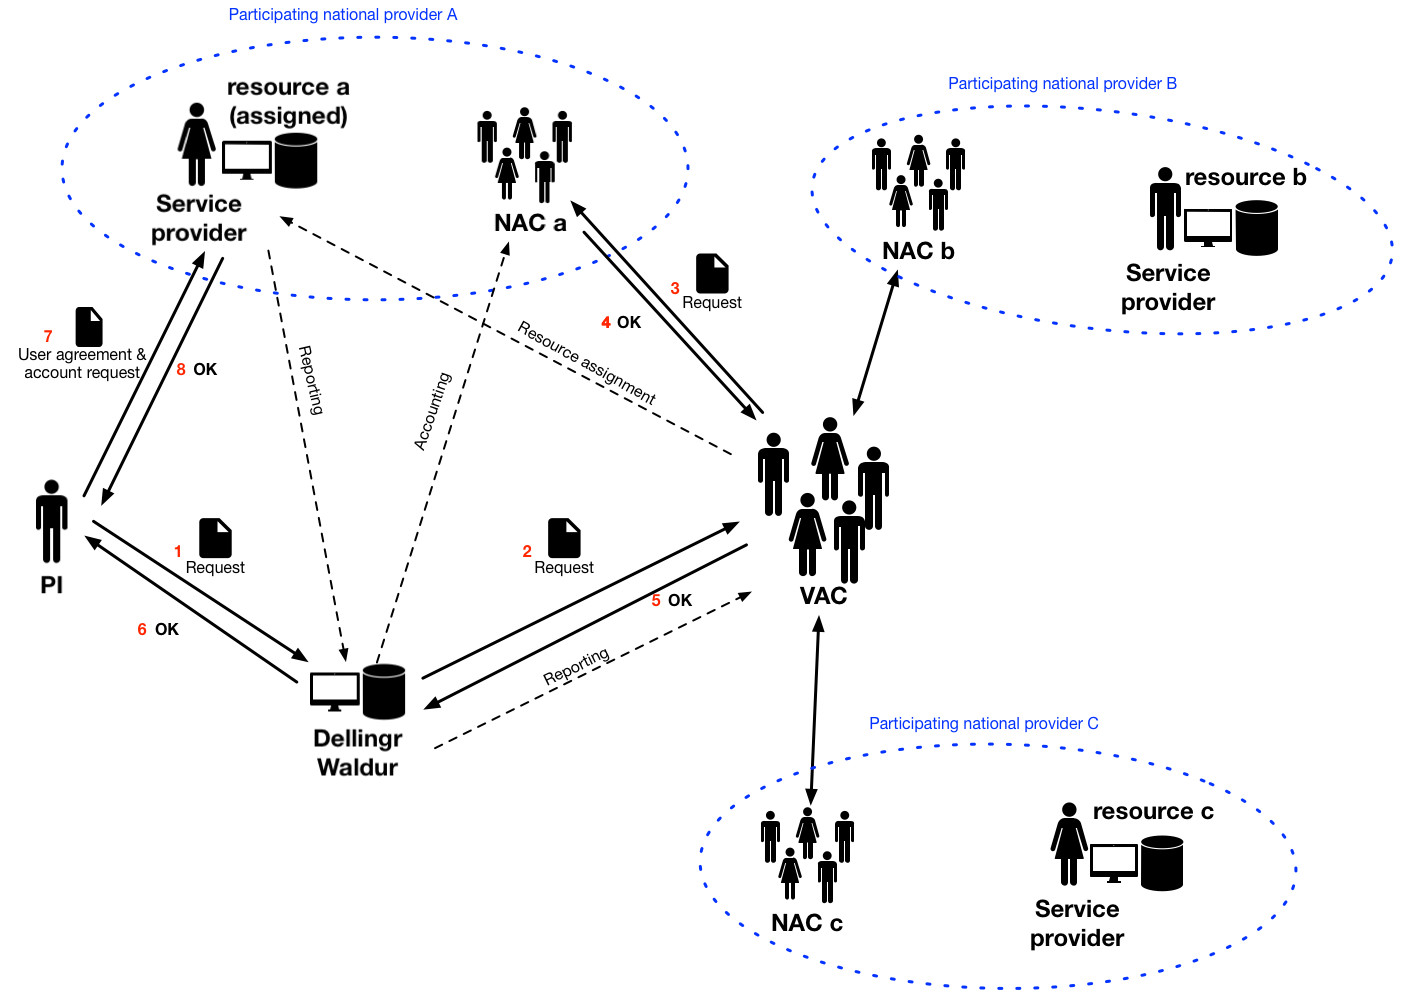
\includegraphics[width=10cm]{Dellingr_pilot2.png}
\caption{Outline of application process.}\label{fig:pilot2_application}
\end{figure}

\end{itemize}

Beyond the request flow, NAC representatives are updating monthly usage by customers of the resources, which affects accounting for the requests. Some screenshots from the process are included below to provide a feeling as to what it looks like for the PI.

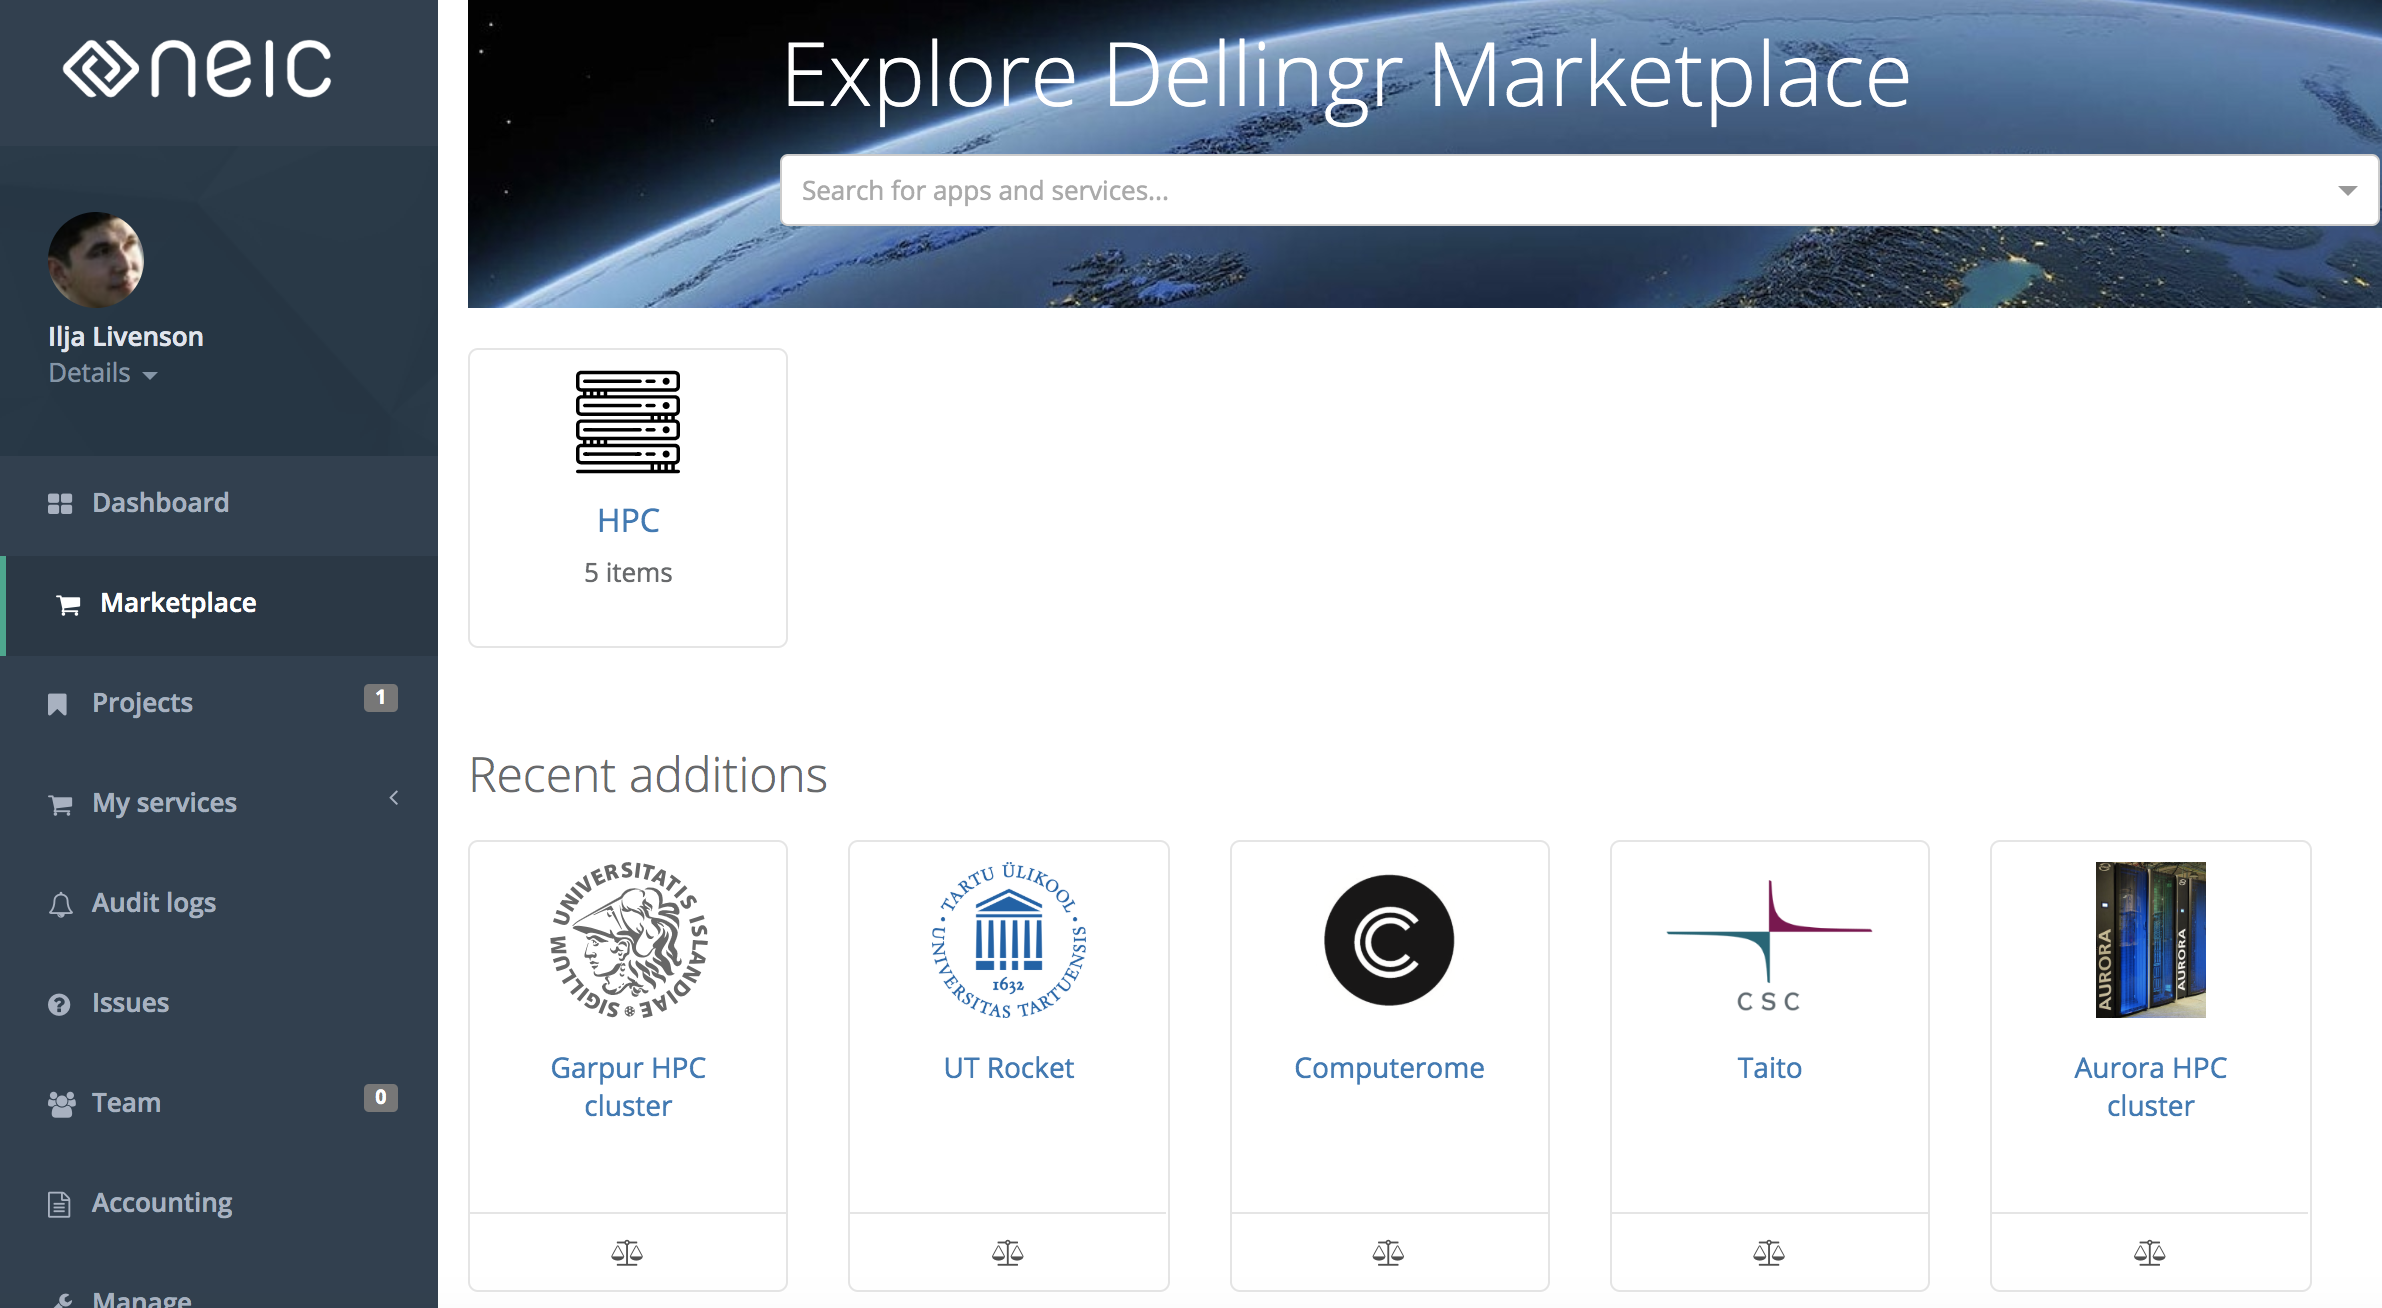
\includegraphics[width=16cm]{images/marketplace.png}

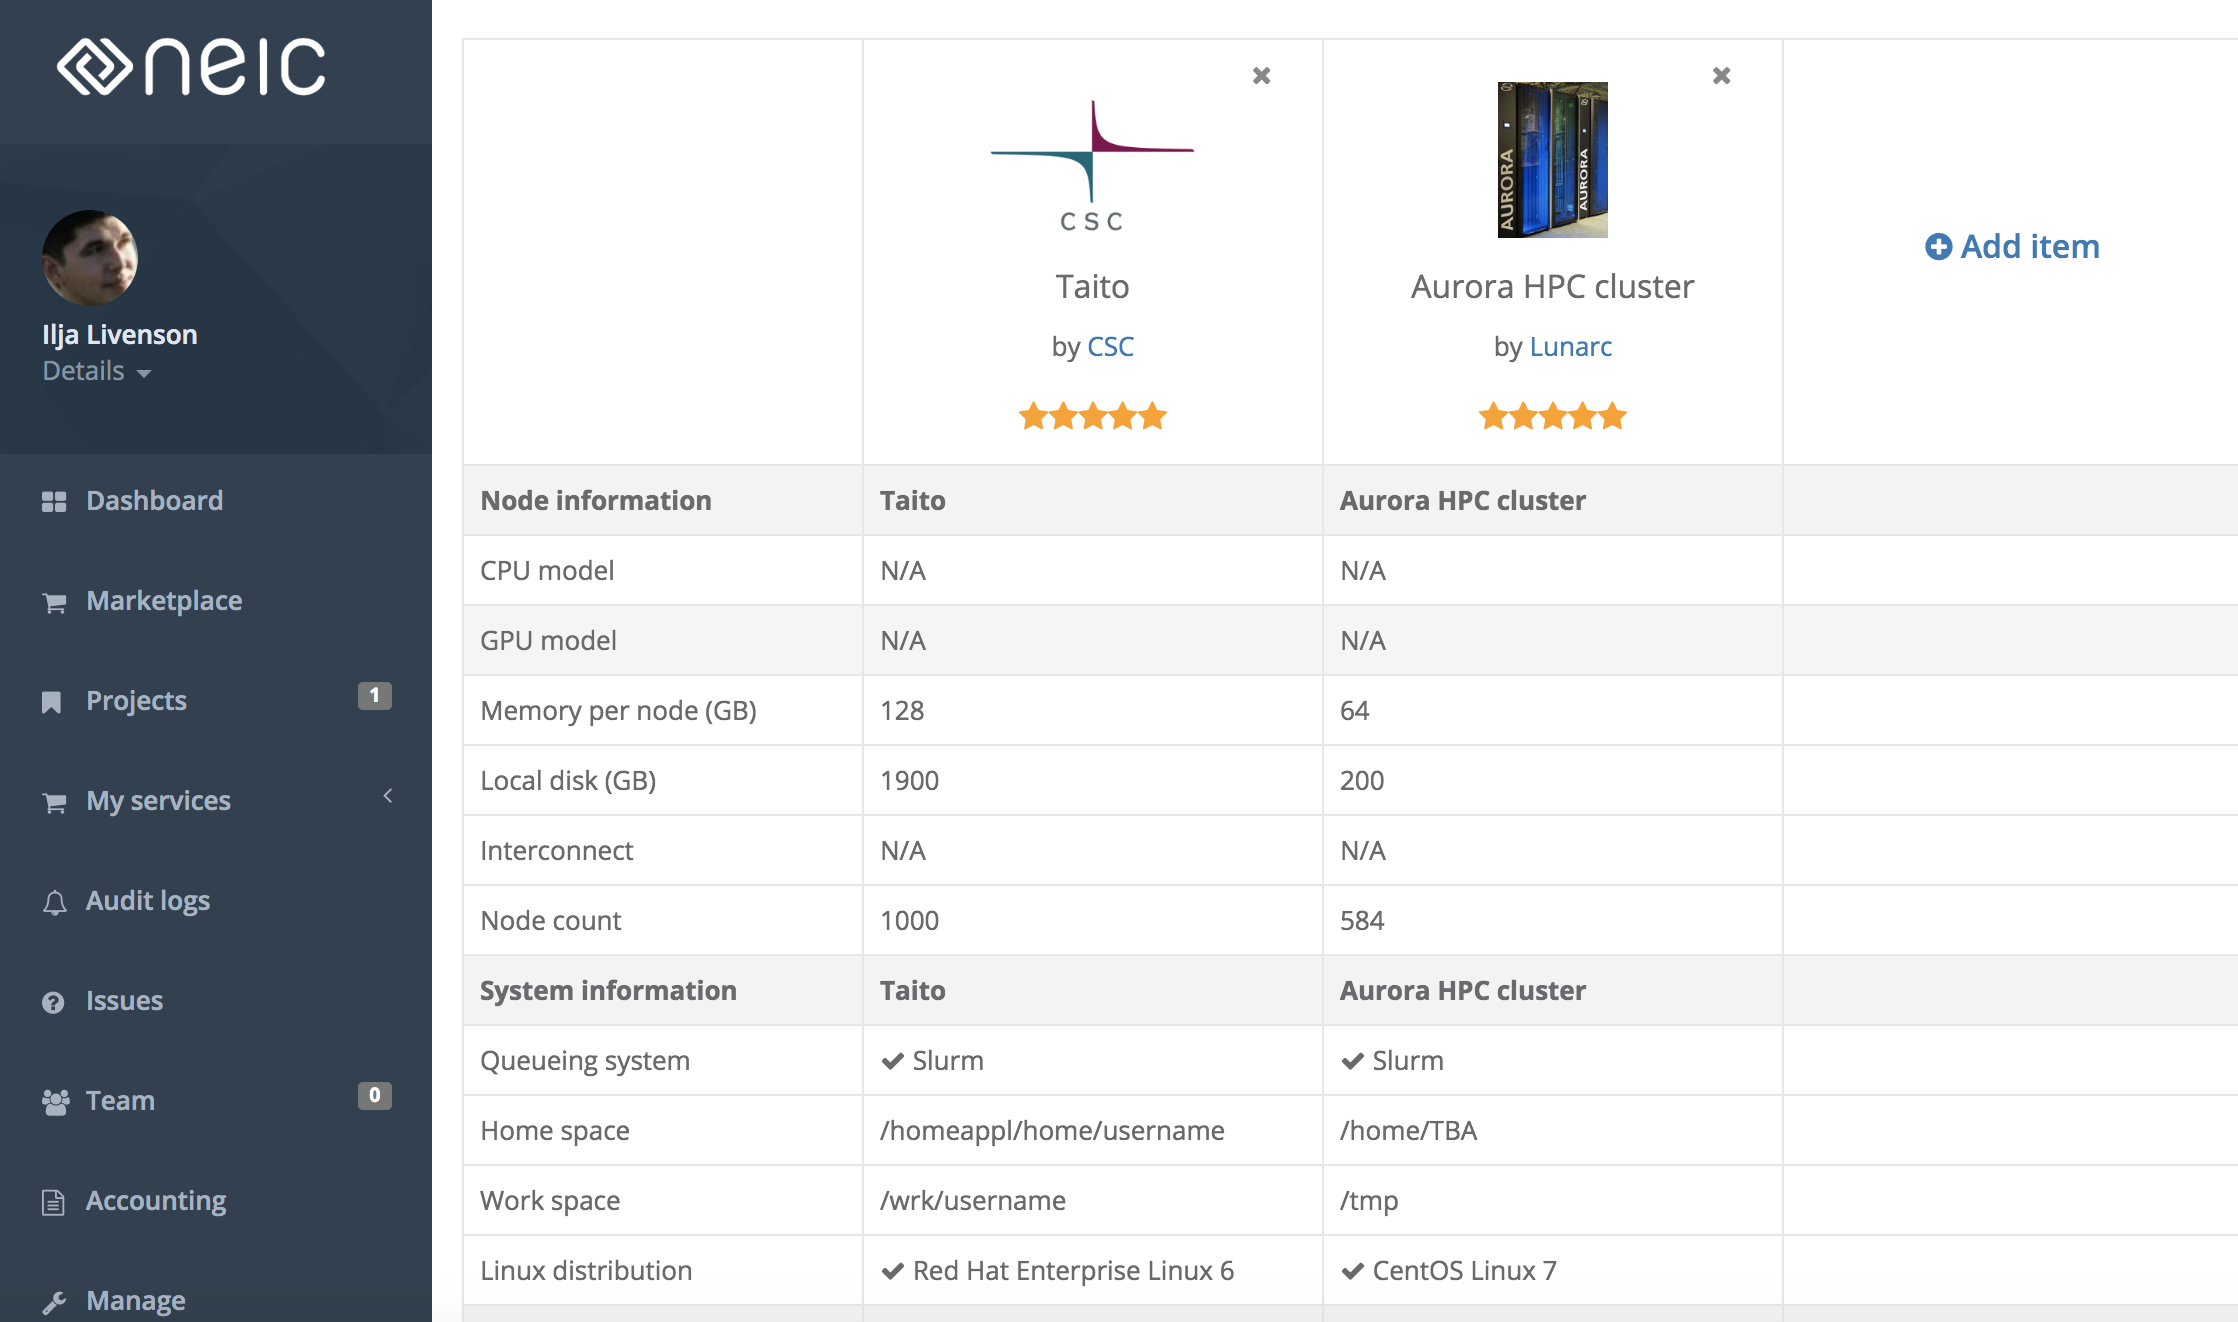
\includegraphics[width=16cm]{images/compare.png}

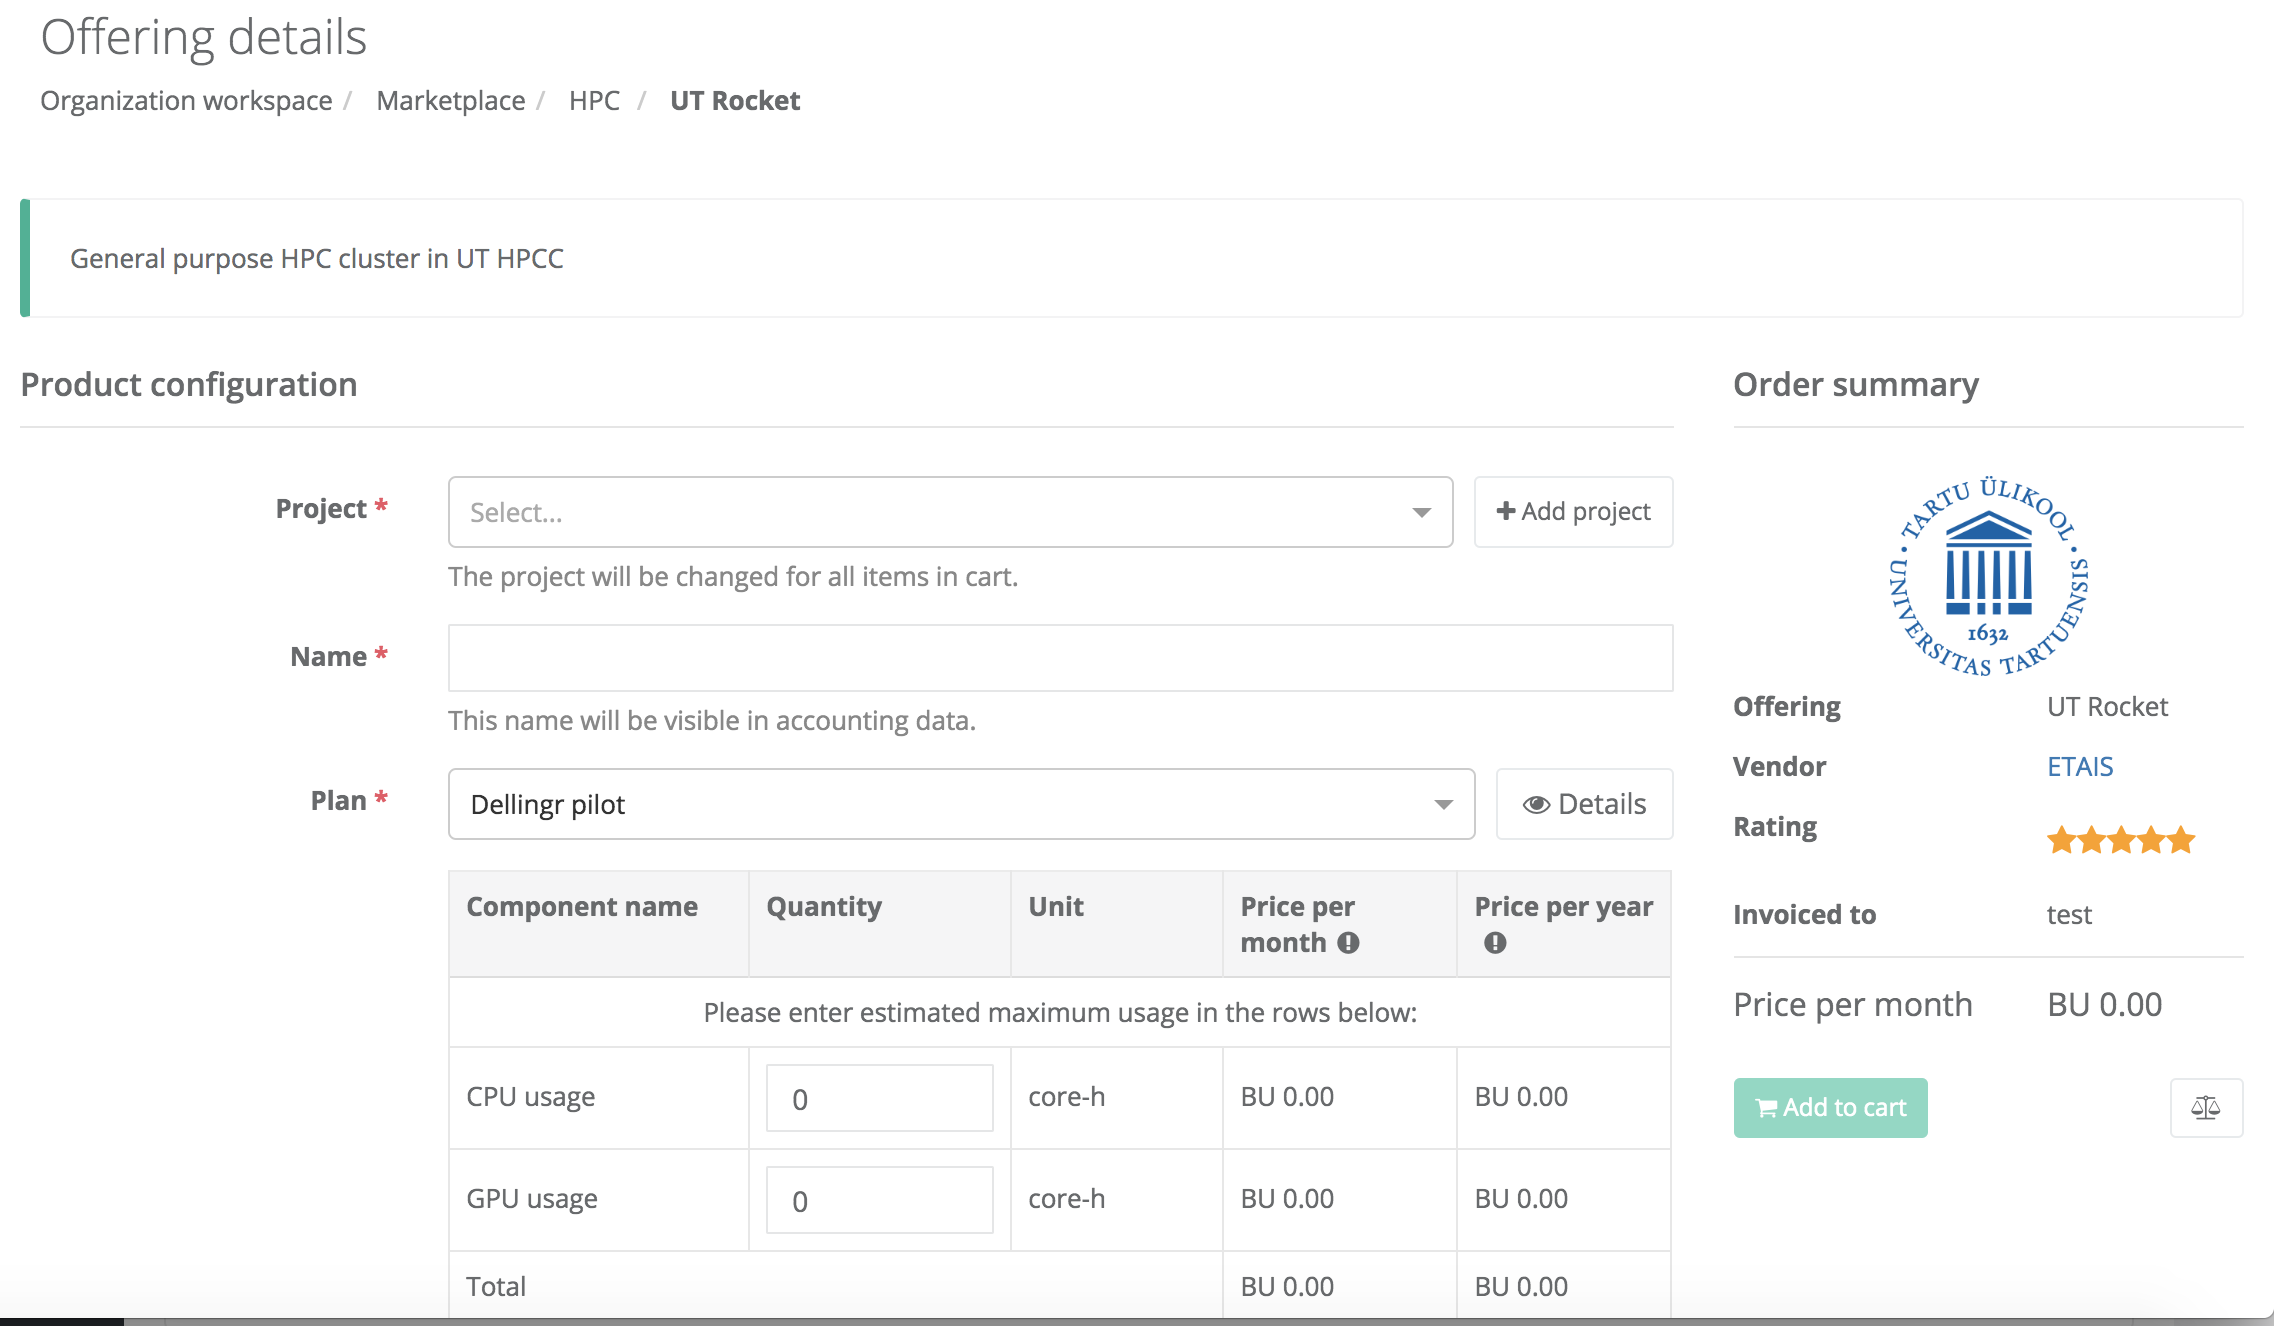
\includegraphics[width=16cm]{images/request.png}

\section{Similar projects and investigations}
\begin{itemize}
    \item []
Other projects with the aim to share resources across national borders exist. 
Although these projects share similarities with \dell in their aim and scope they differ in their implementation. 
\end{itemize}
\subsection{PRACE}
%% \todo[inline]{short paragraph on the PRACE-project}
\bitm
    \item []
The mission of PRACE~\cite{prace}~(Partnership for Advanced Computing in Europe) is to enable high-impact scientific discovery and engineering research and development across all disciplines to enhance European competitiveness for the benefit of society.
PRACE is established as an international not-for-profit association (aisbl) with its seat in Brussels. It has 26 member countries whose representative organisations create a pan-European supercomputing infrastructure, providing access to computing and data management resources and services for large-scale scientific and engineering applications at the highest performance level.
The PRACE Research Infrastructure provides access to HPC systems 
The computer systems (called Tier-0 systems) and their operations that are accessible through PRACE are provided for by 5 PRACE hosting members: BSC representing Spain, CINECA representing Italy, ETH Zurich/CSCS representing Switzerland, GCS representing Germany, and GENCI representing France.

Scientists and researchers can apply for access to PRACE resources. 
Industrial users can apply if they have their head offices or substantial R\&D activity in Europe.
The PRACE Access Committee, composed of leading international scientists and engineers, ranks the proposals received and produces a recommendation to award PRACE resources based on scientific and technical excellence.

For the purposes of comparison to the \dell project, PRACE is able to share \einfra resources (in this case large HPC) across national borders as PRACE is formed as an aisbl~\cite{aisbl}.
Membership of this type of legal entity was judged by tax authorities to not impart a financial gain to the members as outlined in~\cite{prace-aisbl}.
The PRACE aisbl does not buy \einfra resources. 
The PRACE members pay membership fees and hosting members contribute \einfra resources.
By operating under this legal entity and model, the usage of contributed \einfra resources across borders does not attract a VAT payment in the users' country.
\eitm

\subsection{"Meteorology"}
\begin{itemize}
    \item []
The Nordic meteorological agencies of Denmark, Finland, Iceland, Sweden and Norway have charged the firm KPMG to study the practicalities of sharing resources across the Nordics. They have identified three different options of which option 3 is the one that come closest to the proposed \dell implementation. In the option 3 it is stated that VAT is to be added to the cost of the service.

Currently there is a NO/SE/FI cooperation~\cite{metcoop} on running the numerical weather prediction model hardware.
A result of this cooperation is that separate standard forecast models are not run anymore.
Smaller models and research models are still run separately.
\end{itemize}

\section{Summary} 
\label{sec-summary}
\begin{itemize}
    \item []
In summary the following points have been made:

\begin{itemize}
    \item []\textbf{VAT}: \\VAT must be calculated and paid in the country where the "taxable person" is located. 
    \item []\textbf{Access}: \\ Access can in most cases be granted through a federation such as eduGAIN~\cite{edugain}. Remote access for EU-nationals is a non-issue, for non-EU nationals the situation is unclear. 
    \item []\textbf{Licensing}: \\The licensing conditions for the software used is subject to the software provider/copyright holders instructions. 
    \item []\textbf{Cost recovery implementation}:\\ As full cost coverage is necessary and, as VAT must be paid on the full cost of providing the core-hours consumed, an approach for calculating the cost of one core-hour is recommended for the case where the cost of one core-hour is not readily available. 
\end{itemize}

\item [] {\bf A proposal to share resources across national borders}. \\
This proposal aims to be in accordance with resource allocation and sharing policies of \nps and VAT regulations. 

A project or programme could be set up over a fixed amount of time e.g. 2~or 3~years.
Within this timeframe, the interested \nps of \einfra (both HPC and Cloud) would pledge over shorter time-scales \einfra resources that can be provided to external (international) users.
For example over a 2~year project there could be four 6~month time slice pledges or six 4~month pledges.
Setting up such a programme over a fixed schedule with shorter time-scales for the resource pledges aims to address the concerns of some collaboration members that \einfra resources cannot be shared internationally in a permanent fashion.
A permanent or open-ended \einfra resource sharing programme would violate the primary reason some \nps are granted money nationally in order to primarily serve the interests of national research organizations (i.e. universities) and researchers.
Also, a programme composed of resource pledges divided into time slices would allow to correct any resource usage/sharing imbalances.
These could be corrected by changing the resource pledges for subsequent time slices.

The resource sharing between nations would be facilitated using the tools and procedures developed in the project i.e the {\nolinebreak {\url{https://share.neic.no}}} framework and the concept that members of national allocation committees work together as a Virtual Allocation Committee.

The Waldur framework, tested in the Dellingr project, is used to handle the resource requests from users and to gather the accounting information from the hosting \nps.
Invoices for resource usage can be issued by hosting \nps to the research projects or institutes of the users.
The hosting \nps are free to not insist that the before-tax total for the \einfra usage is be paid, but the invoice functions as a vehicle for the local VAT payment.
This invoicing process allows the payable VAT to be paid in the country where the ``taxable person" is located, satisfying local regulations where applicable.

\end{itemize}

\newpage
\bibliography{main}{}
\bibliographystyle{unsrt}

\newpage
\begin{appendices}
\newpage
\section{Author Information}
\label{app:authors}
\begin{tabular}{lll}
{\bf Name} & {\bf email address} & {\bf ORCID} \\
% Anna Jonna {\'A}rmannsd{\'o}ttir & {\tt annaj@hi.is} & 
Mathias Br{\"a}nnvall & {\tt mathias.brannvall@it.uu.se}; & 0000-0003-4979-4123 \\
Juha Fagerholm & {\tt juha.fagerholm@csc.fi} & 0000-0002-9972-4468 \\
Jens Svalgaard Kohrt & {\tt svalgaard@sdu.dk} & 0000-0002-3104-0406 \\
Ivar Koppel & {\tt ivar.koppel@ut.ee} & 0000-0002-5617-4785 \\
% Bj{\o}rn Lindi & {\tt bjorn.lindi@ntnu.no} &  \\
Ilja Livenson & {\tt ilja.livenson@ut.ee} & 0000-0002-4011-8367 \\
Petri Nikunen & {\tt petri.nikunen@csc.fi} & 0000-0003-0759-6372 \\
Ahti Saar & {\tt Ahti.Saar@ut.ee} & 0000-0003-0642-961X \\
Anders Sj{\"o}str{\"o}m & {\tt Anders.Sjostrom@lunarc.lu.se} & 0000-0003-2213-2138 \\
Hj{\"o}rleifur Sveinbj{\"o}rnsson & {\tt hs@hi.is} &  0000-0002-4120-1234 \\
%% M{\'a}ni Mar{\'i}us Vi{\dh}arsson & {\tt mani@hi.is} &  \\
John White & {\tt john.white@cern.ch} & 0000-0001-5614-0895 \\
\end{tabular}


\end{appendices}
\end{document}
